\section{Experimental Results}

\subsection{Prediction Performance}
Table~\ref{tab:pred_perf} summarizes macro performance in a multi-seed benchmark ($n=10$), reporting mean and standard deviation. Random Forest and LSTM obtained the lowest average errors, while the proposed SNN remained competitive and substantially more stable than the MLP baseline.

\begin{table}[!h]
\caption{Multi-seed multimodal prediction performance (macro metrics).}
\label{tab:pred_perf}
\centering
\footnotesize
\setlength{\tabcolsep}{3pt}
\begin{tabular}{lccc}
\toprule
Model & MAE macro & RMSE macro & $R^2$ macro \\
\midrule
Random Forest & $\mathbf{0.409 \pm 0.062}$ & $0.557 \pm 0.086$ & $\mathbf{0.335 \pm 0.131}$ \\
LSTM & $0.428 \pm 0.059$ & $\mathbf{0.548 \pm 0.073}$ & $0.313 \pm 0.139$ \\
SNN (proposed) & $0.447 \pm 0.064$ & $0.566 \pm 0.072$ & $0.291 \pm 0.146$ \\
MLP & $0.781 \pm 0.193$ & $0.983 \pm 0.178$ & $-5.460 \pm 5.220$ \\
\bottomrule
\end{tabular}
\end{table}

Although Random Forest achieved the lowest MAE, the SNN demonstrated competitive predictive performance while enabling deployment on low-power edge devices, which is essential for remote environmental monitoring scenarios. The ranking indicates that the SNN is not the lowest-error model in absolute terms, but it remains in a competitive range with materially better robustness than MLP in this small-data regime. In paired sign tests (SNN vs Random Forest), p-values were 0.3438 (MAE), 1.0000 (RMSE), and 1.0000 ($R^2$), indicating no statistically significant global superiority at $\alpha=0.05$.

\subsection{Model Ranking Visualization}
Figure~\ref{fig:mae_models_sba} provides a compact visual ranking of macro MAE across models, with variability bars from the multi-seed protocol. The plot confirms that Random Forest and LSTM form the lowest-error group, SNN remains in the same practical range for edge deployment, and MLP presents substantially higher variance and error in this dataset regime.

\begin{figure}[!htbp]
\centering
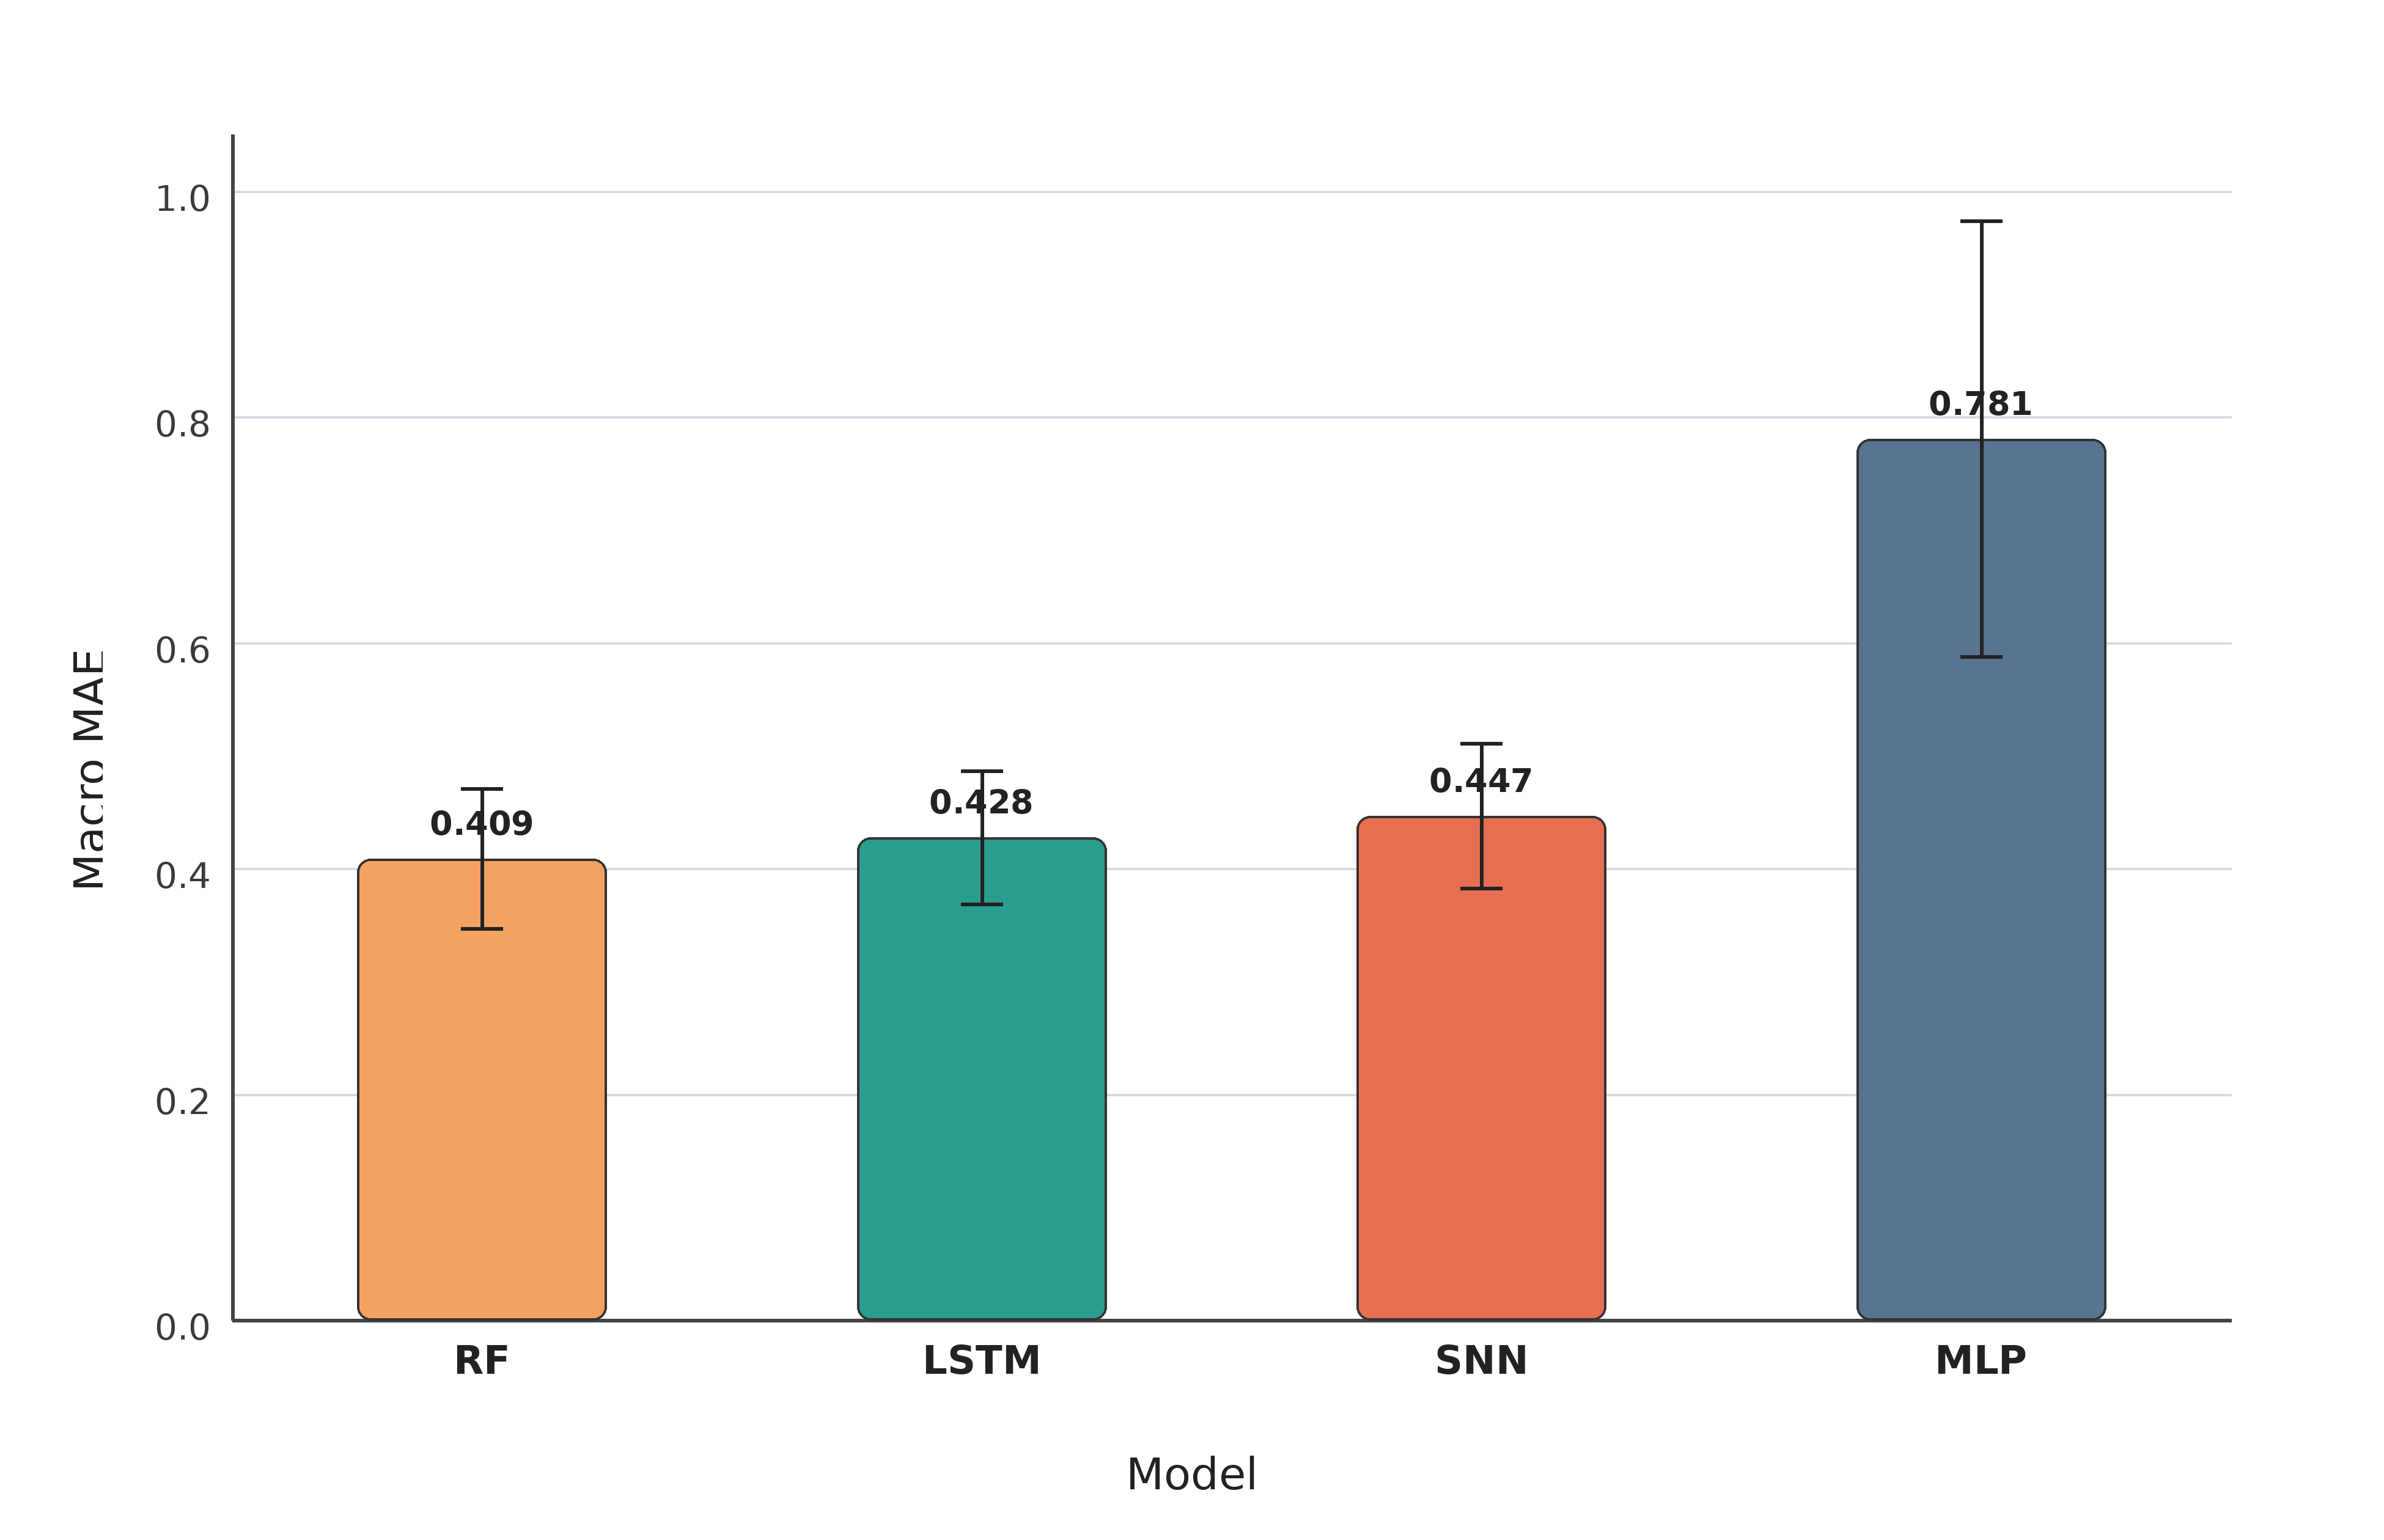
\includegraphics[width=0.98\linewidth]{mae_vs_model_bar.png}
\caption{Comparative macro MAE across multimodal models (mean with standard deviation bars).}
\label{fig:mae_models_sba}
\end{figure}

\subsection{Augmentation Ablation}
To quantify augmentation impact, we compared SNN training with no augmentation (factor 1) and augmentation $\times 10$ (Gaussian noise, $\sigma=0.01$) under the same protocol across five seeds (7, 13, 21, 42, 84). Augmentation reduced macro MAE from $0.496 \pm 0.060$ to $0.483 \pm 0.075$ (2.53\% reduction), with slight macro $R^2$ improvement ($0.254 \rightarrow 0.256$) and nearly unchanged macro RMSE ($0.615 \rightarrow 0.617$). The most relevant per-target gain was for turbidity MAE ($1.139 \rightarrow 1.102$), supporting augmentation as a practical stabilization strategy for this dataset size.

\begin{figure}[!htbp]
\centering
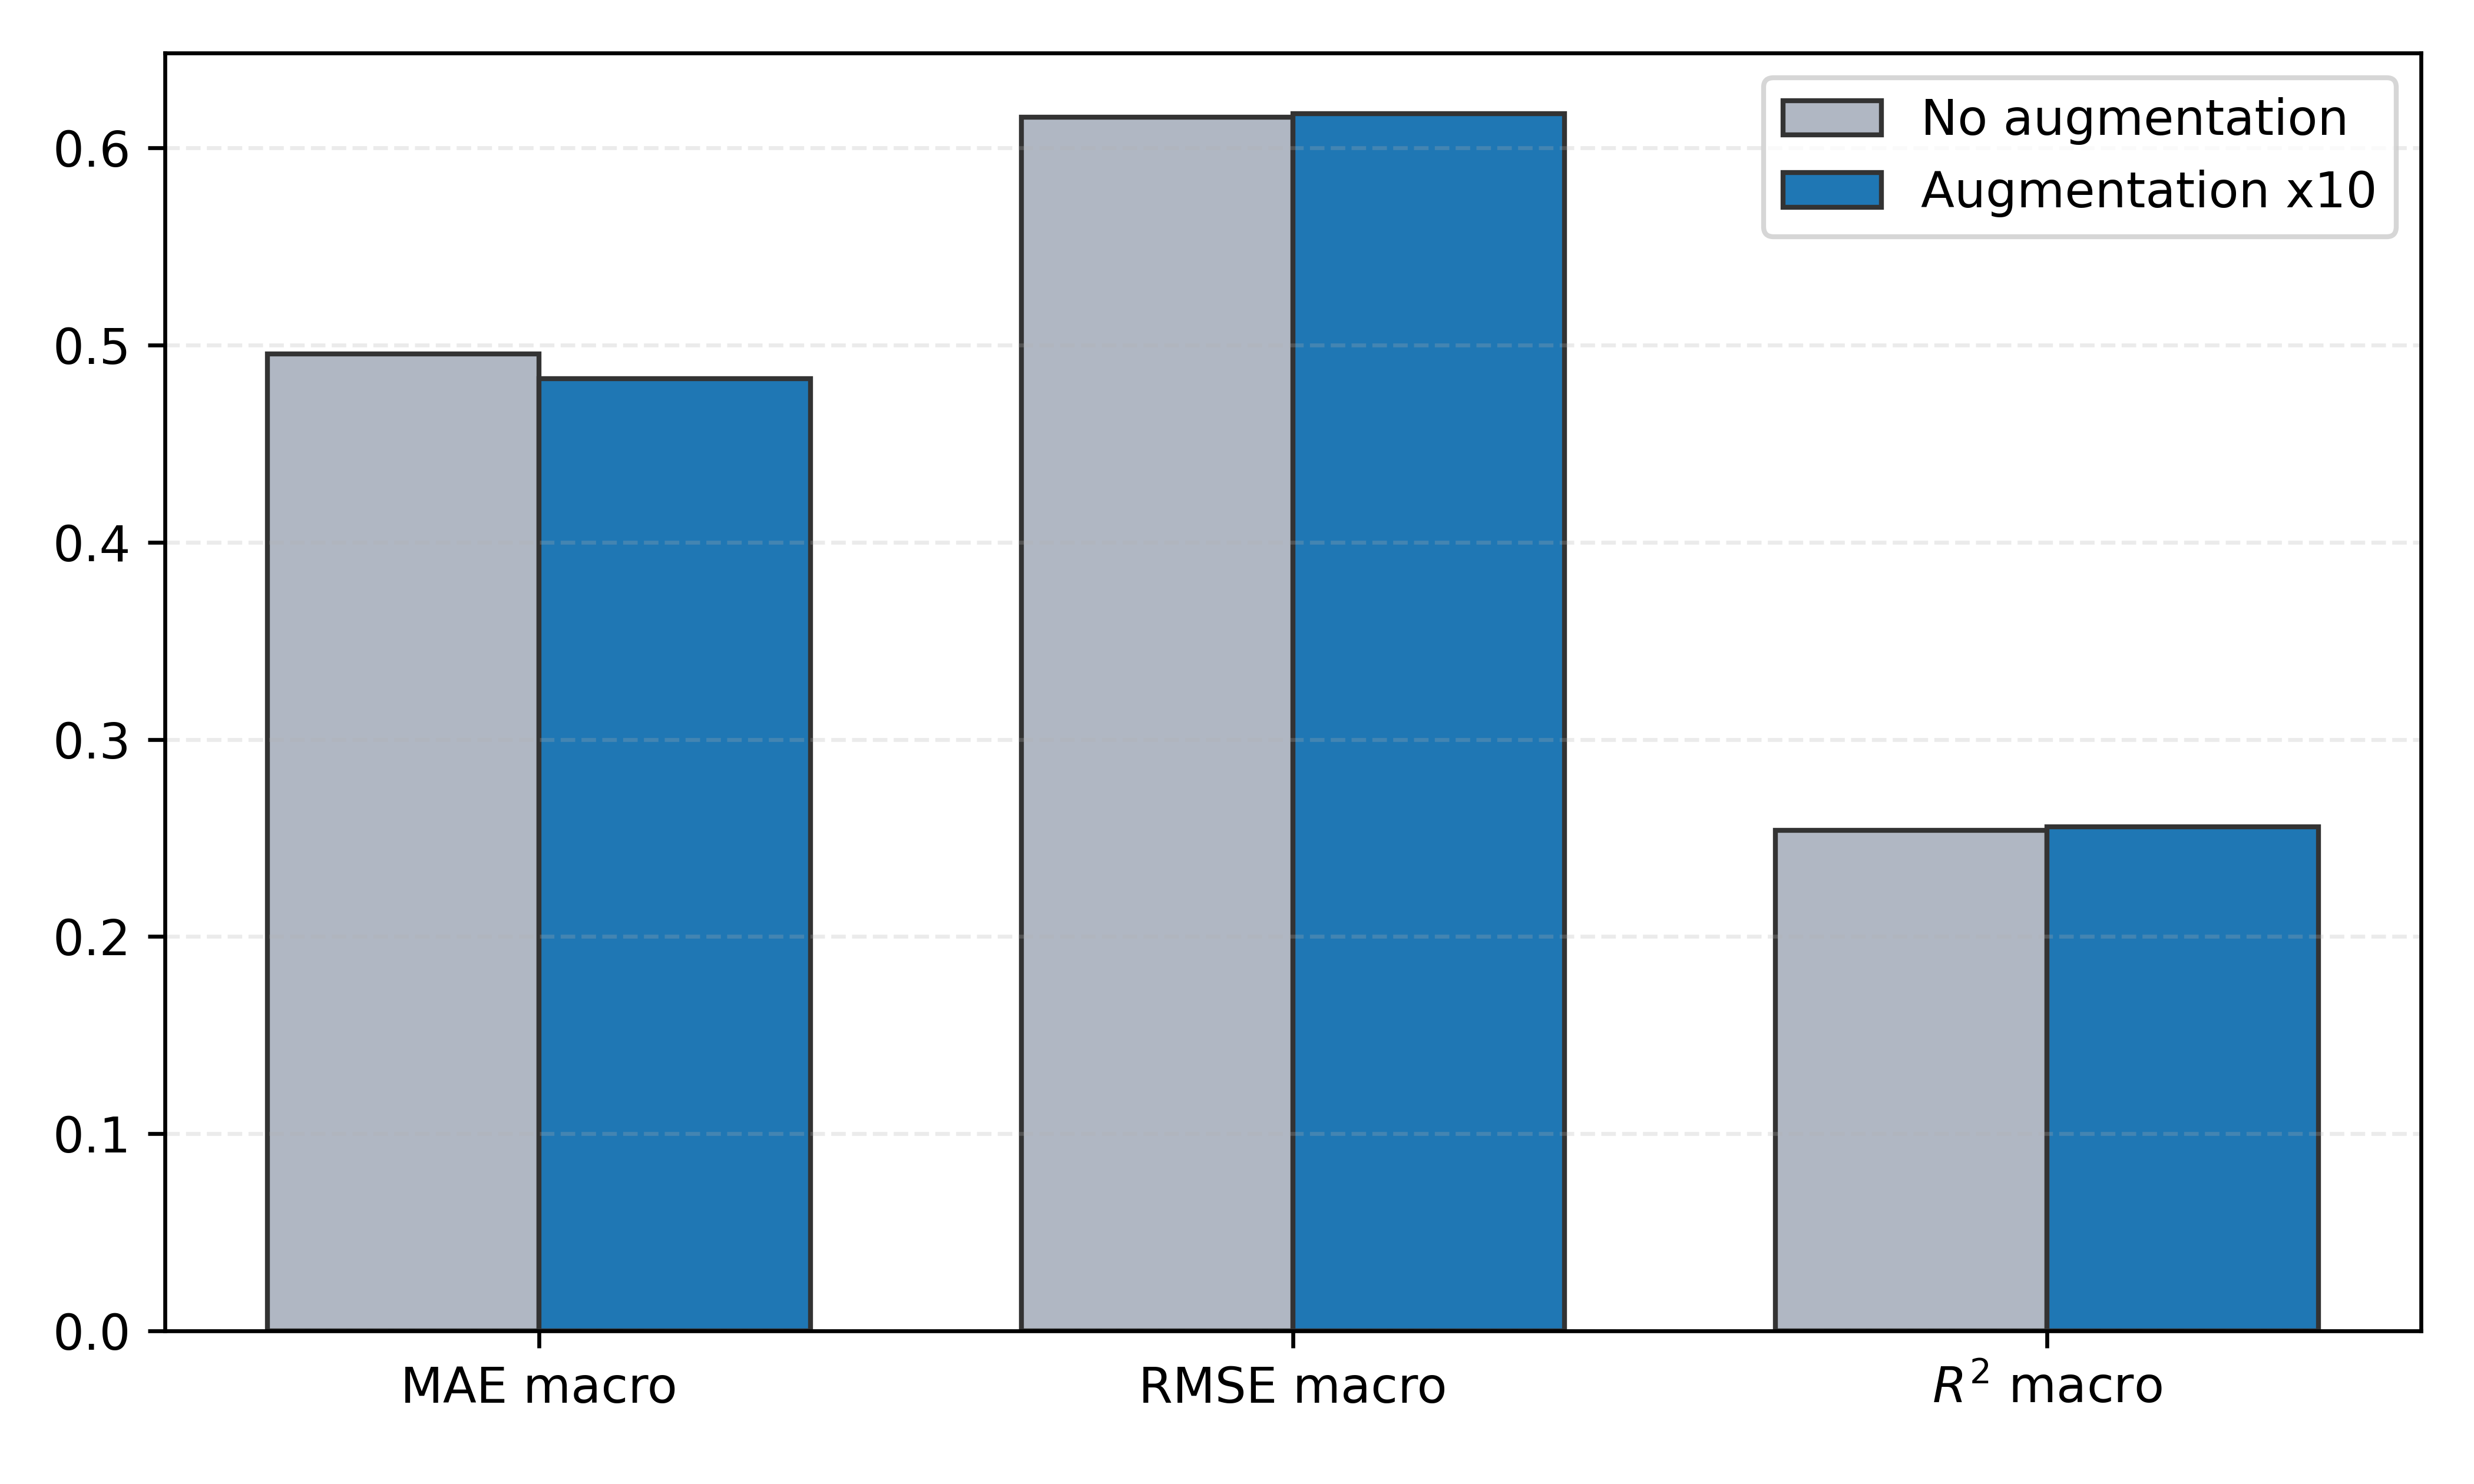
\includegraphics[width=0.95\linewidth]{augmentation_ablation_bar.png}
\caption{Augmentation ablation (5 seeds): no augmentation vs augmentation $\times 10$ for macro metrics.}
\label{fig:aug_ablation_sba}
\end{figure}

\subsection{Target-Weight Sensitivity}
Because turbidity is the most difficult target, we also evaluated a small loss-weight sweep in the SNN to quantify the trade-off between global fit and TURB-focused optimization. Table~\ref{tab:snn_weight_sweep_sba} shows that increasing TURB weight can reduce $MAE_{TURB}$, but with a slight decrease in global $R^2$.

\begin{table}[!htbp]
\caption{SNN loss-weight sweep (10 seeds).}
\label{tab:snn_weight_sweep_sba}
\centering
\footnotesize
\setlength{\tabcolsep}{3pt}
\begin{tabular}{lccc}
\toprule
Weights (pH, OD, TURB) & MAE macro & MAE TURB & $R^2$ macro \\
\midrule
$(0.20,\,0.20,\,0.60)$ & $\mathbf{0.447}$ & $1.012$ & $\mathbf{0.291}$ \\
$(0.15,\,0.15,\,0.70)$ & $0.452$ & $1.022$ & $0.289$ \\
$(0.10,\,0.10,\,0.80)$ & $0.454$ & $1.028$ & $0.288$ \\
$(0.05,\,0.15,\,0.80)$ & $0.448$ & $\mathbf{1.006}$ & $0.280$ \\
\bottomrule
\end{tabular}
\end{table}

\subsection{Predicted-vs-True Behavior}
Figure~\ref{fig:pred_true_multi_sba} complements aggregate metrics by showing point-wise agreement between predicted and observed values for each target. pH and OD concentrate closer to the identity line, while turbidity presents larger spread, consistent with its higher error contribution in previous tables.

\begin{figure}[!htbp]
\centering
\begin{minipage}{0.32\linewidth}
\centering
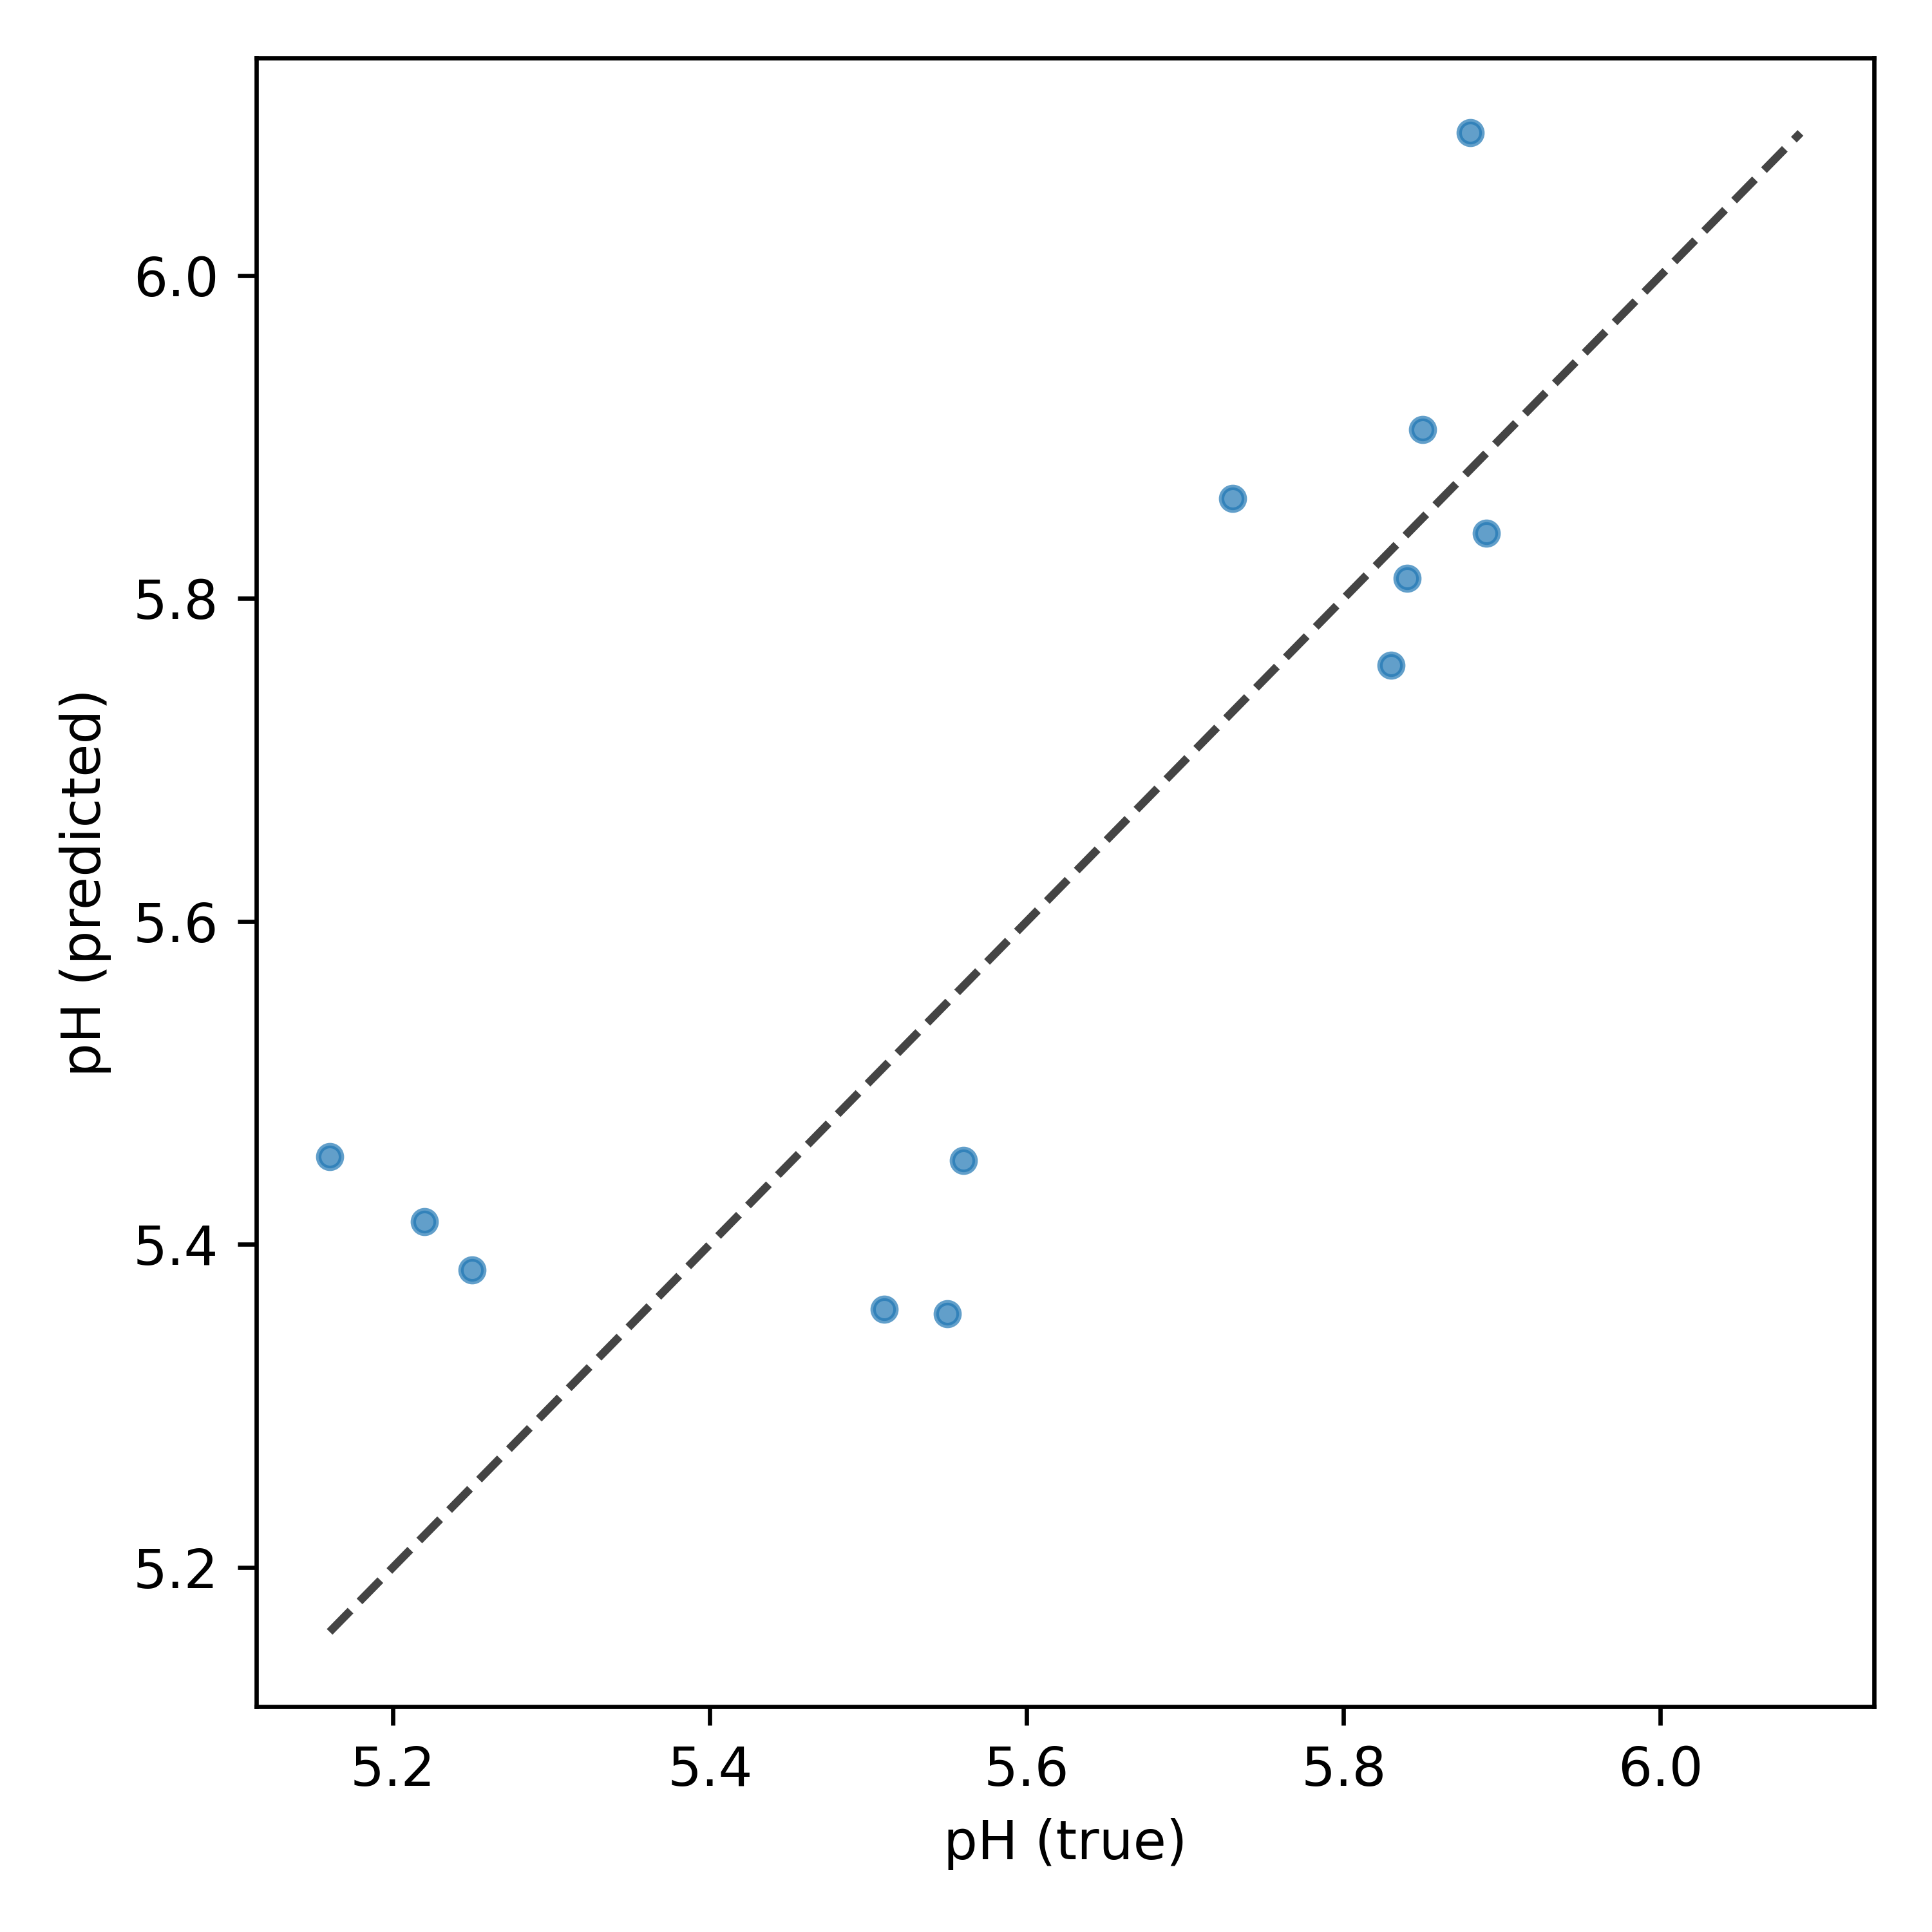
\includegraphics[width=\linewidth]{pred_vs_real_pH_multi.png}
\par\vspace{1mm}{\footnotesize (a) pH\par}
\end{minipage}\hfill
\begin{minipage}{0.32\linewidth}
\centering
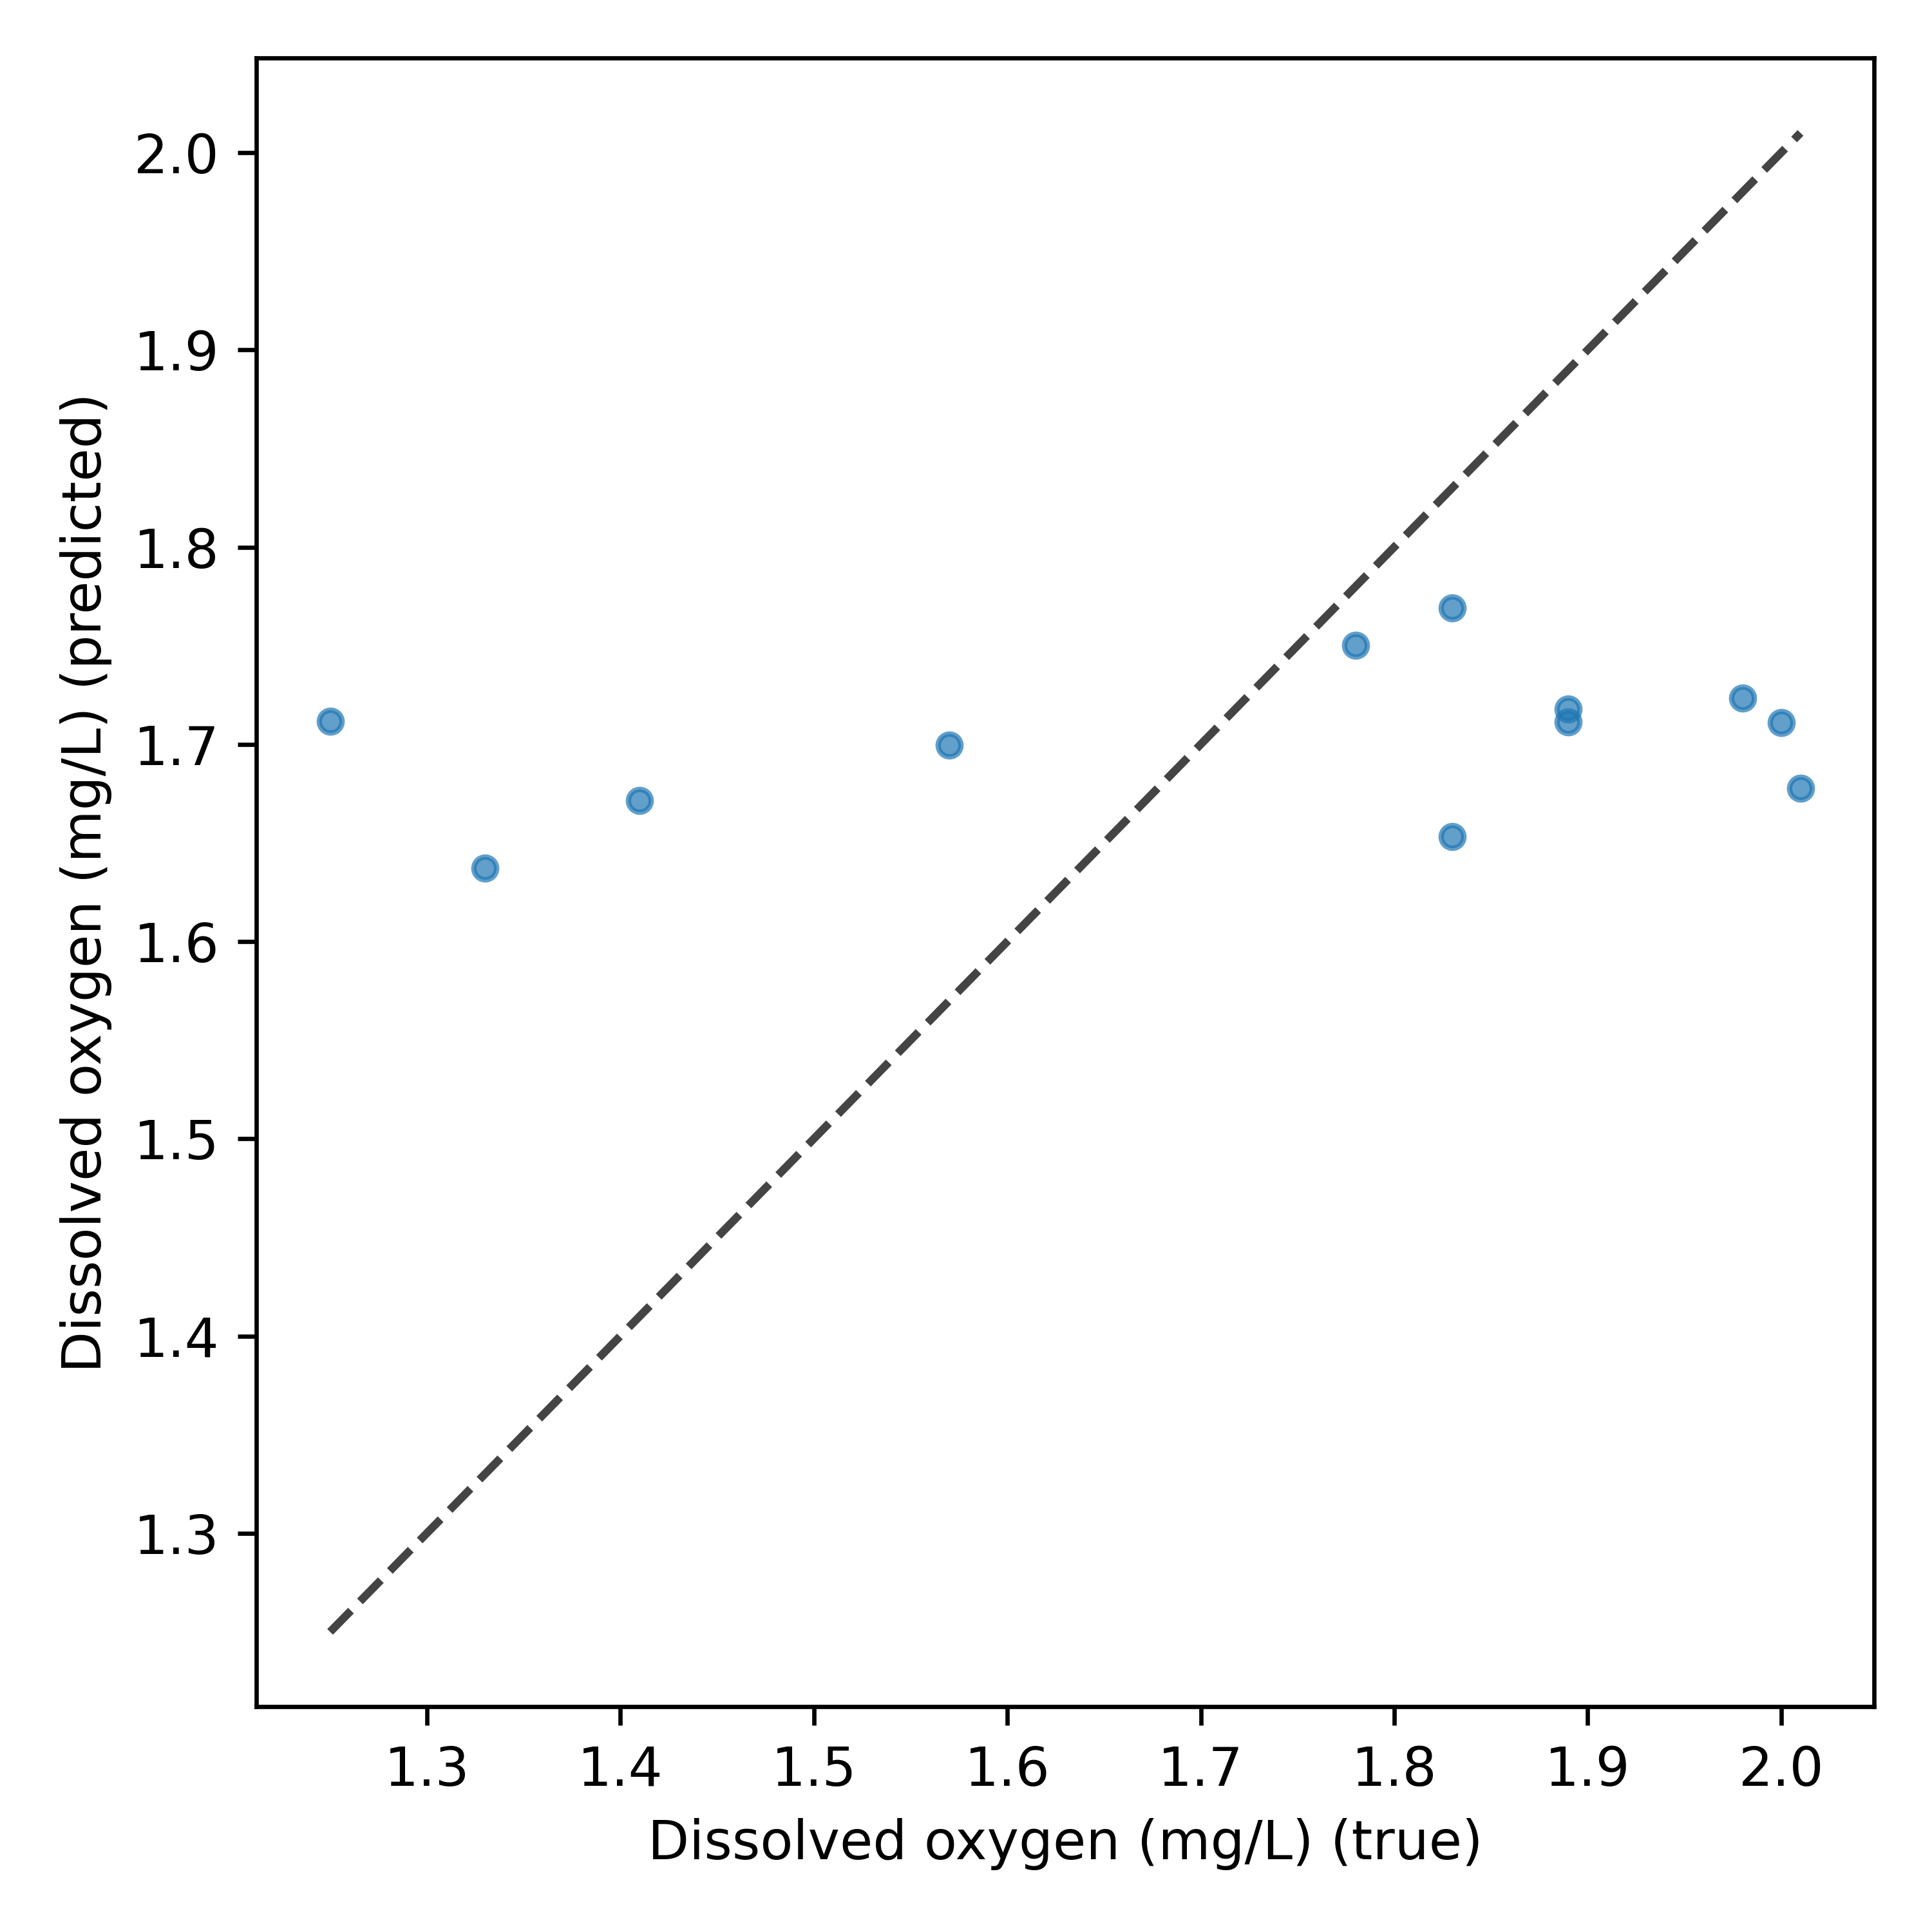
\includegraphics[width=\linewidth]{pred_vs_real_OD_multi.png}
\par\vspace{1mm}{\footnotesize (b) OD\par}
\end{minipage}\hfill
\begin{minipage}{0.32\linewidth}
\centering
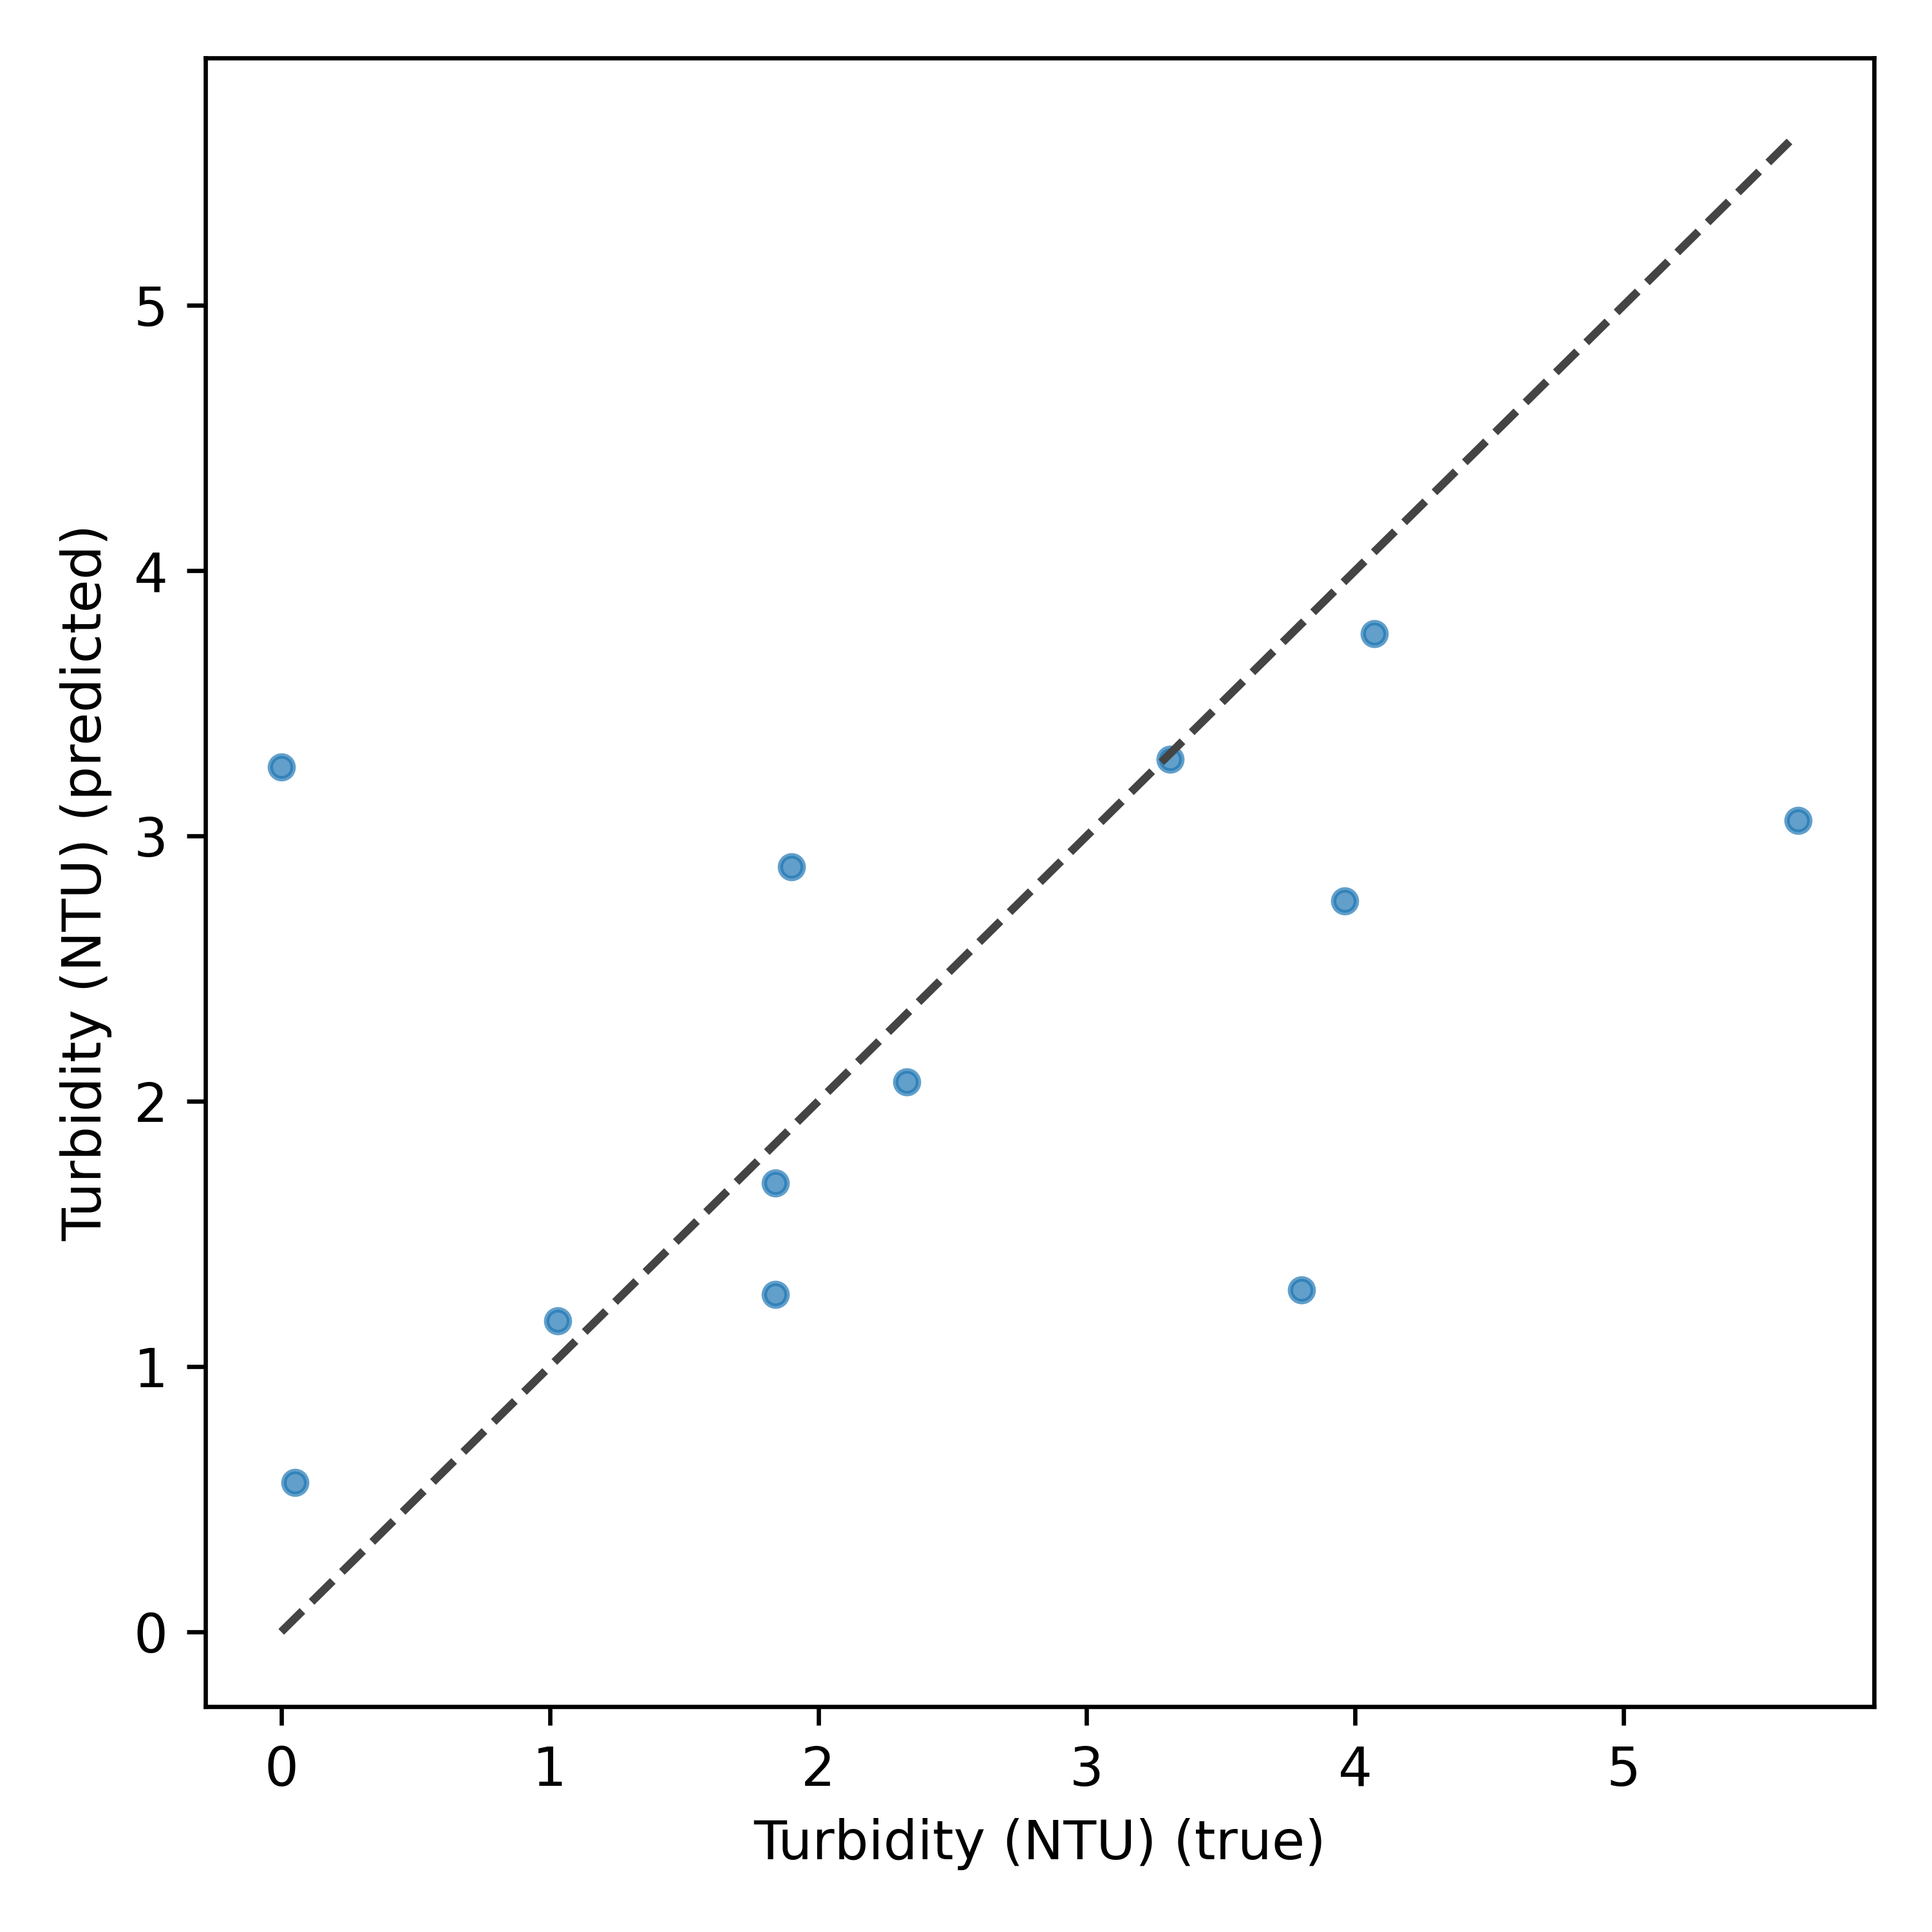
\includegraphics[width=\linewidth]{pred_vs_real_TURB_multi.png}
\par\vspace{1mm}{\footnotesize (c) TURB\par}
\end{minipage}
\caption{Predicted vs. true values in the multimodal SNN for pH, dissolved oxygen, and turbidity.}
\label{fig:pred_true_multi_sba}
\end{figure}

\subsection{Spatial Results and Pollution Index}
IDW interpolation was used to convert point predictions into continuous spatial surfaces, improving environmental interpretation beyond point-wise metrics. As shown in Figure~\ref{fig:idw_combined_sba}, the resulting maps highlight nonuniform spatial behavior across pH, dissolved oxygen, and turbidity, and indicate candidate micro-zones for prioritized field inspection.

\begin{figure}[!htbp]
\centering
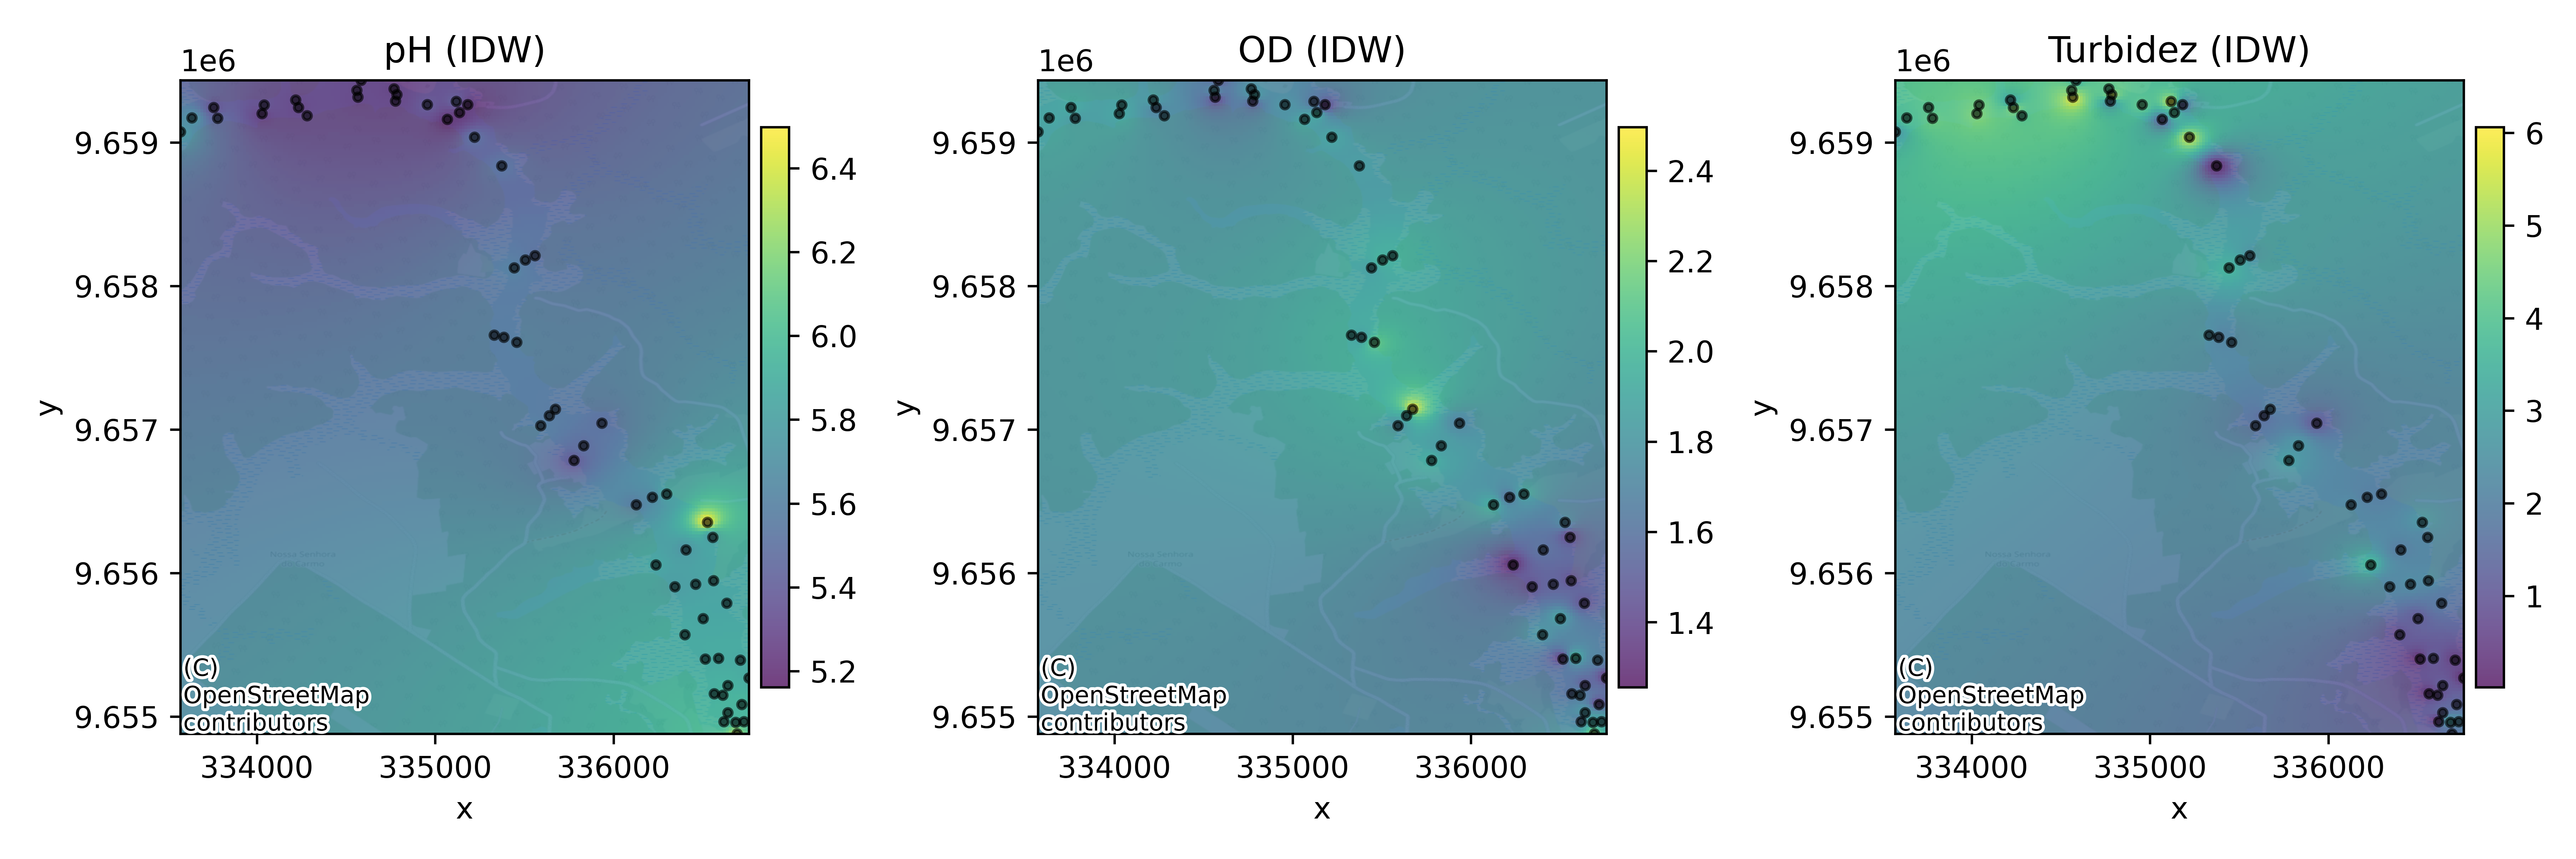
\includegraphics[width=0.98\linewidth]{idw_combined.png}
\caption{IDW interpolated surfaces for pH, dissolved oxygen, and turbidity from sampled points.}
\label{fig:idw_combined_sba}
\end{figure}

To support operational screening, a composite pollution index was computed from multimodal predictions and normalized to $[0,1]$, where higher values indicate worse relative condition within the analyzed set. As illustrated in Figure~\ref{fig:pollution_sba}, the point-level representation and its IDW spatial estimate over the OSM basemap provide a direct visual tool for identifying critical areas.

\begin{figure}[!htbp]
\centering
\begin{minipage}[t]{0.48\linewidth}
\centering
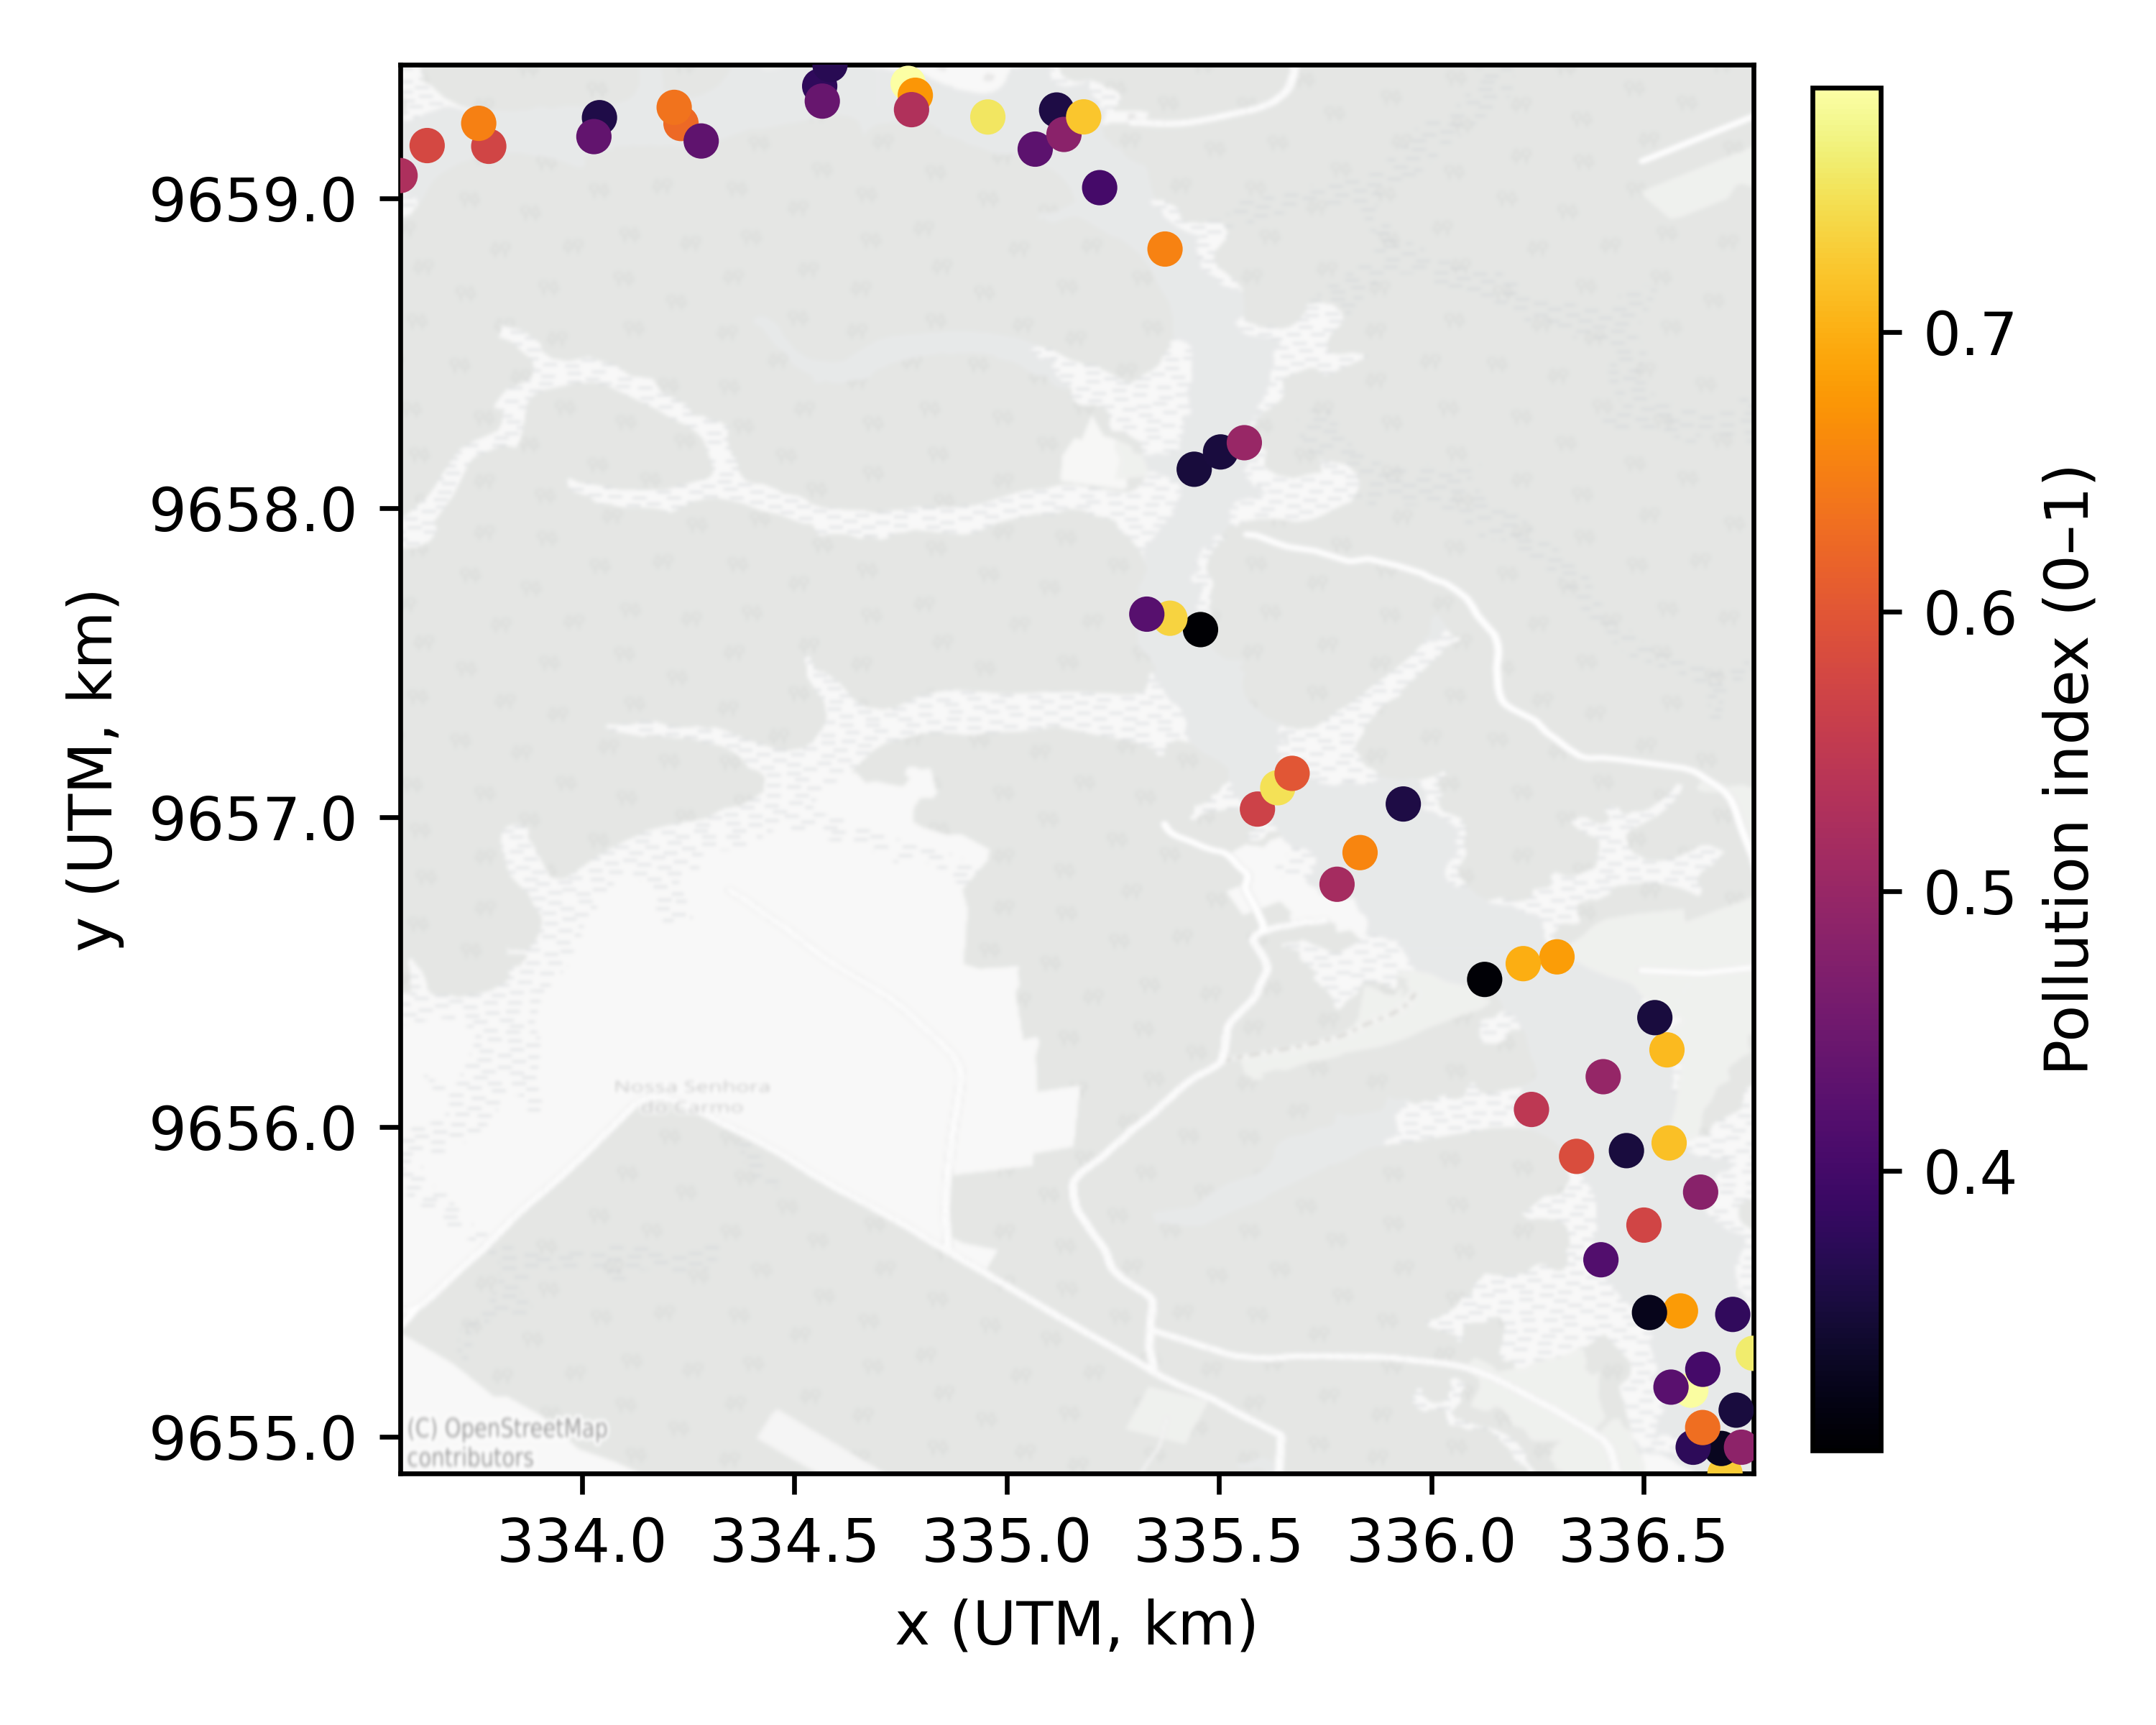
\includegraphics[width=\linewidth]{pollution_scatter.png}
\par\vspace{1mm}{\footnotesize (a) Pollution index at sample points.\par}
\end{minipage}\hfill
\begin{minipage}[t]{0.48\linewidth}
\centering
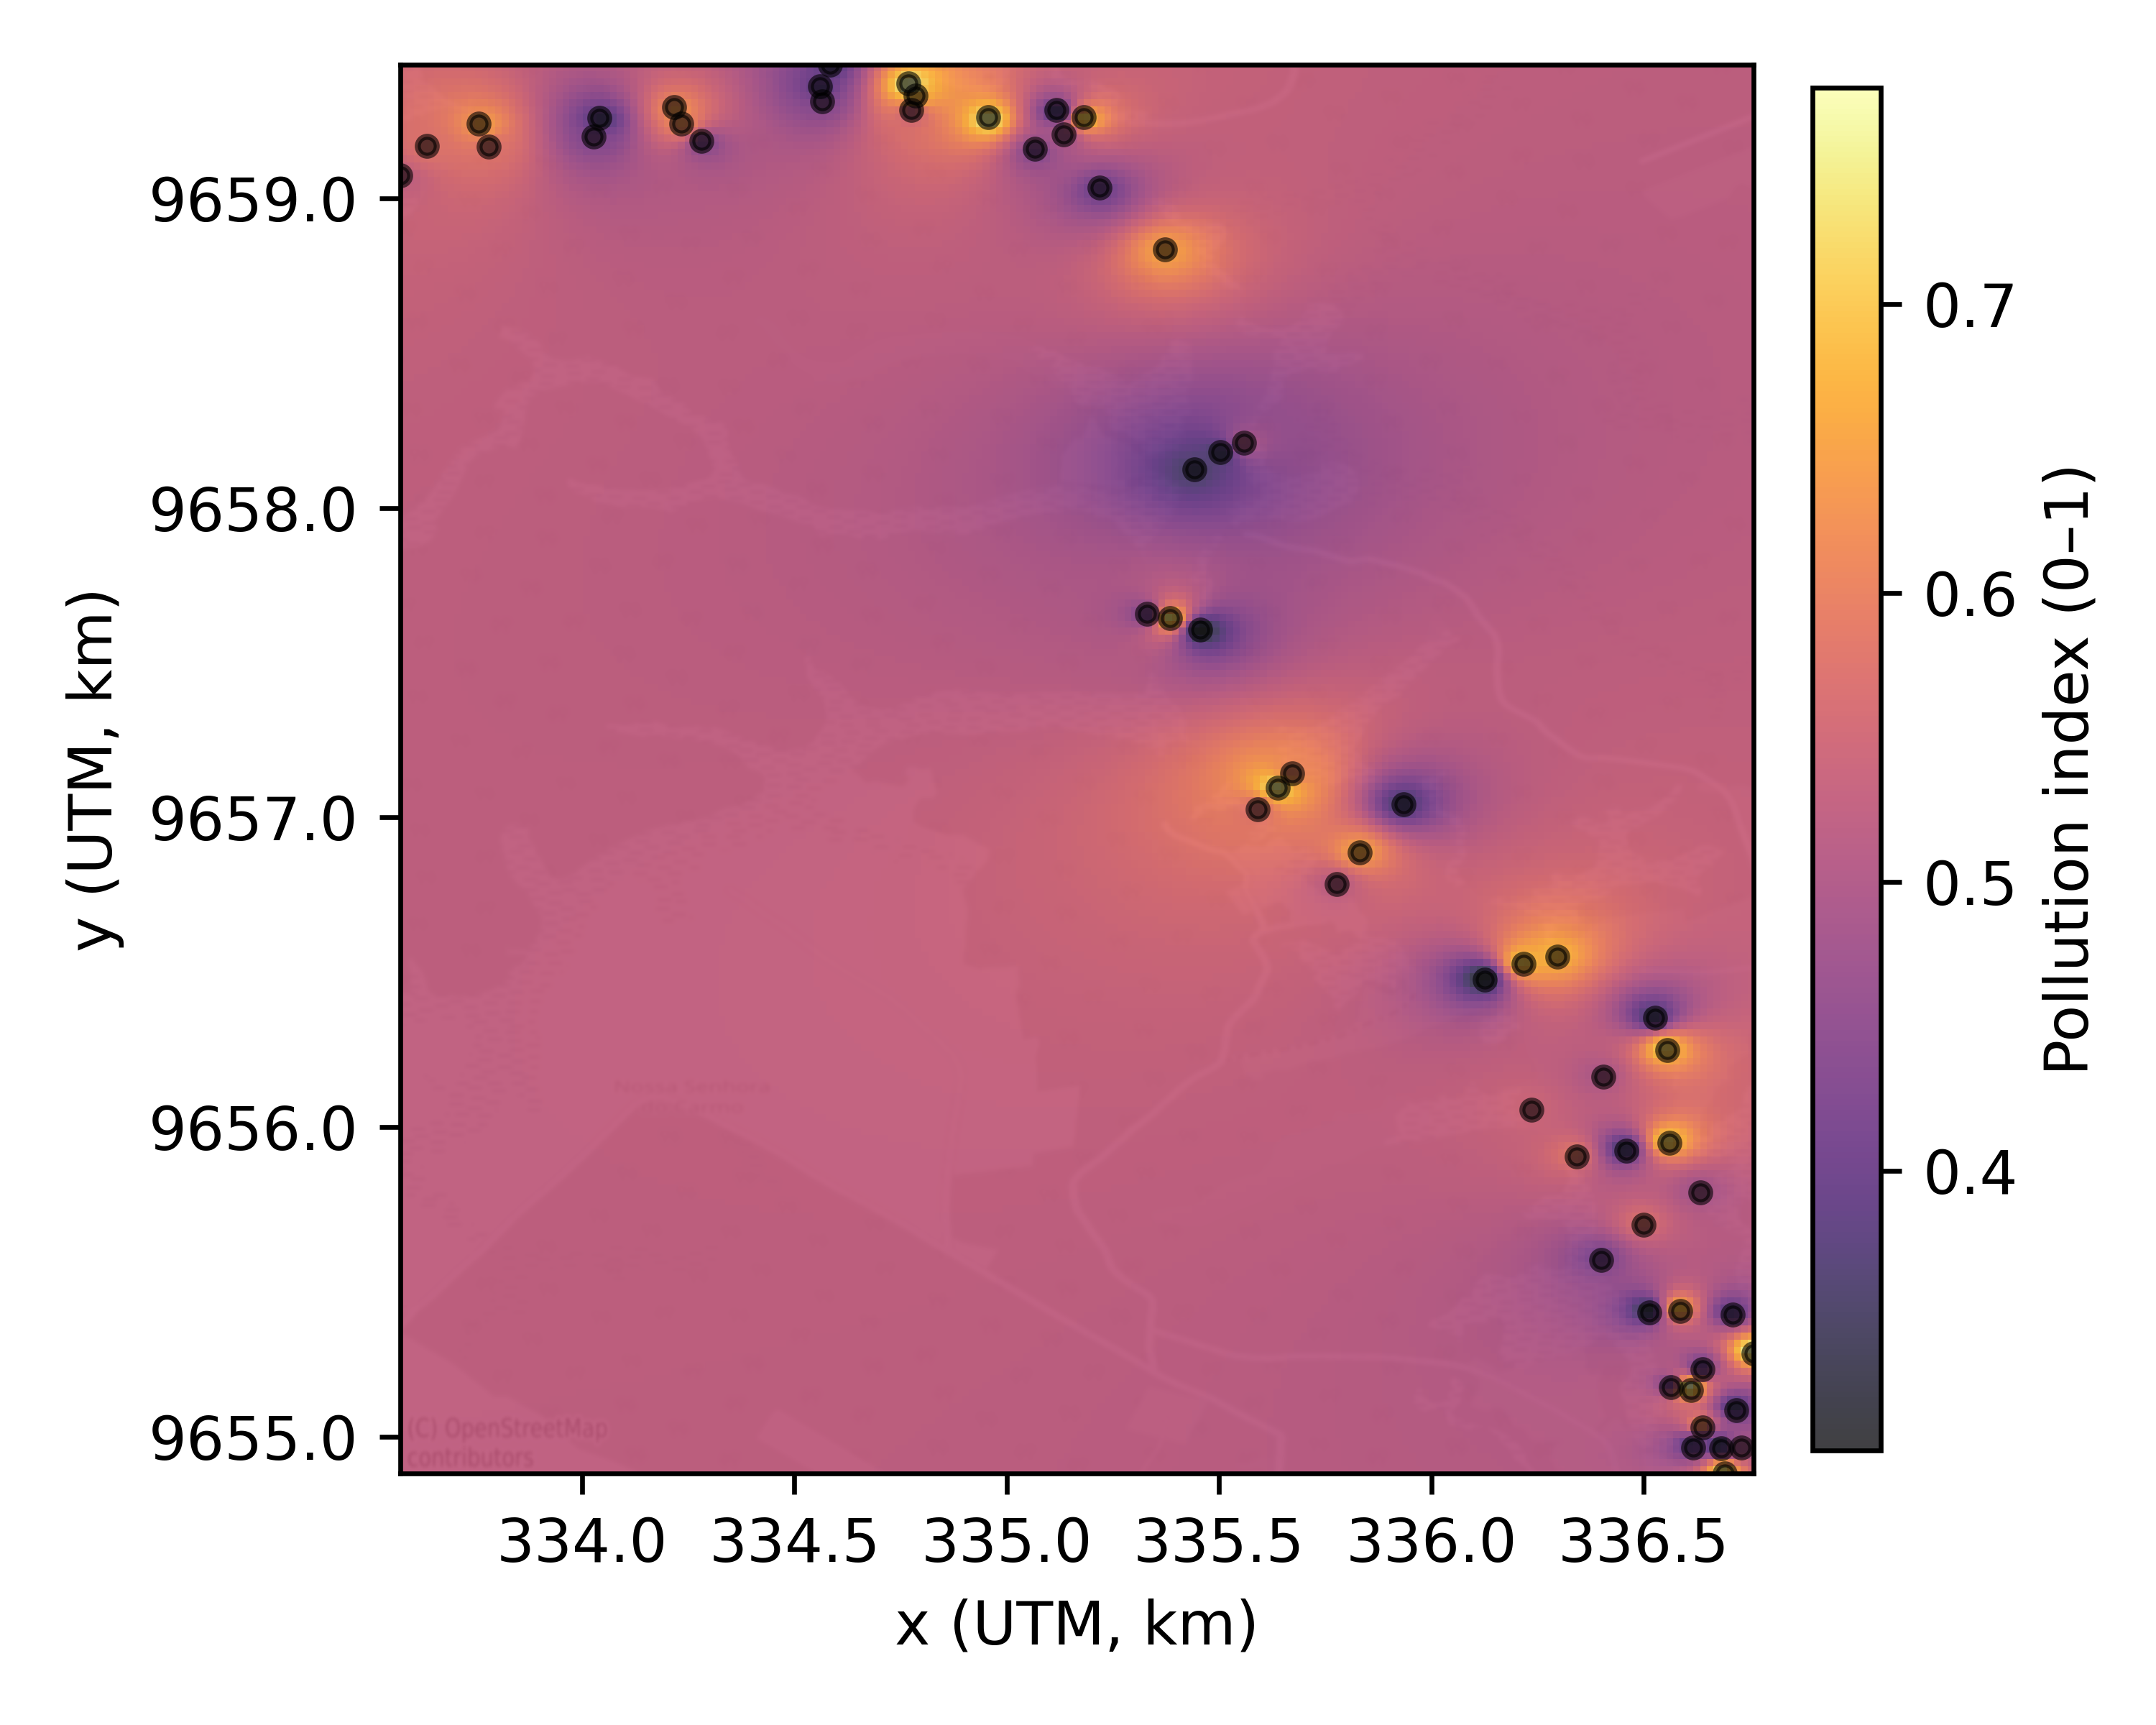
\includegraphics[width=\linewidth]{pollution_idw.png}
\par\vspace{1mm}{\footnotesize (b) IDW surface of the index.\par}
\end{minipage}
\caption{Spatial estimate of the composite pollution index from multimodal predictions (normalized scale $[0, 1]$) over an OpenStreetMap basemap (UTM 21S).}
\label{fig:pollution_sba}
\end{figure}

\subsection{Energy Consumption and Latency}
Table~\ref{tab:energy_latency} reports incremental energy-per-inference and throughput across deployment platforms. ESP32 is feasible for low-rate autonomous scenarios but has higher energy per inference due to limited throughput. Raspberry Pi and Android devices provide much lower mJ/inf in high-throughput settings.

\begin{table}[!htbp]
\caption{Latency/throughput and incremental energy across platforms.}
\label{tab:energy_latency}
\centering
\footnotesize
\setlength{\tabcolsep}{3pt}
\begin{tabular}{lccc}
\toprule
Platform & Thr. (samples/s) & $\Delta P$ (W) & $E$ (mJ/inf) \\
\midrule
ESP32 (MicroPy) & 5.0 & 0.056 & 11.204 \\
Raspberry Pi 4B & 4670.50 & 0.239 & 0.0512 \\
Android A & 12337.40 & 0.128 & 0.0104 \\
Android B & 30905.08 & 0.468 & 0.0151 \\
Android C & 16121.71 & 0.046 & 0.00285 \\
\bottomrule
\end{tabular}
\end{table}

Figure~\ref{fig:energy_bar_lnncs} compares the incremental energy per inference across deployment platforms using a logarithmic scale to preserve visual readability despite large magnitude differences. The plot shows that ESP32 has the highest energy cost per prediction, mainly due to its low throughput, while Raspberry Pi and Android devices operate in a much lower mJ/inf range. Among mobile platforms, the figure also highlights that higher throughput does not always imply lower energy per inference, reinforcing that platform selection should be based on the joint analysis of processing speed and incremental power behavior under real deployment conditions.

\begin{figure}[!htbp]
\centering
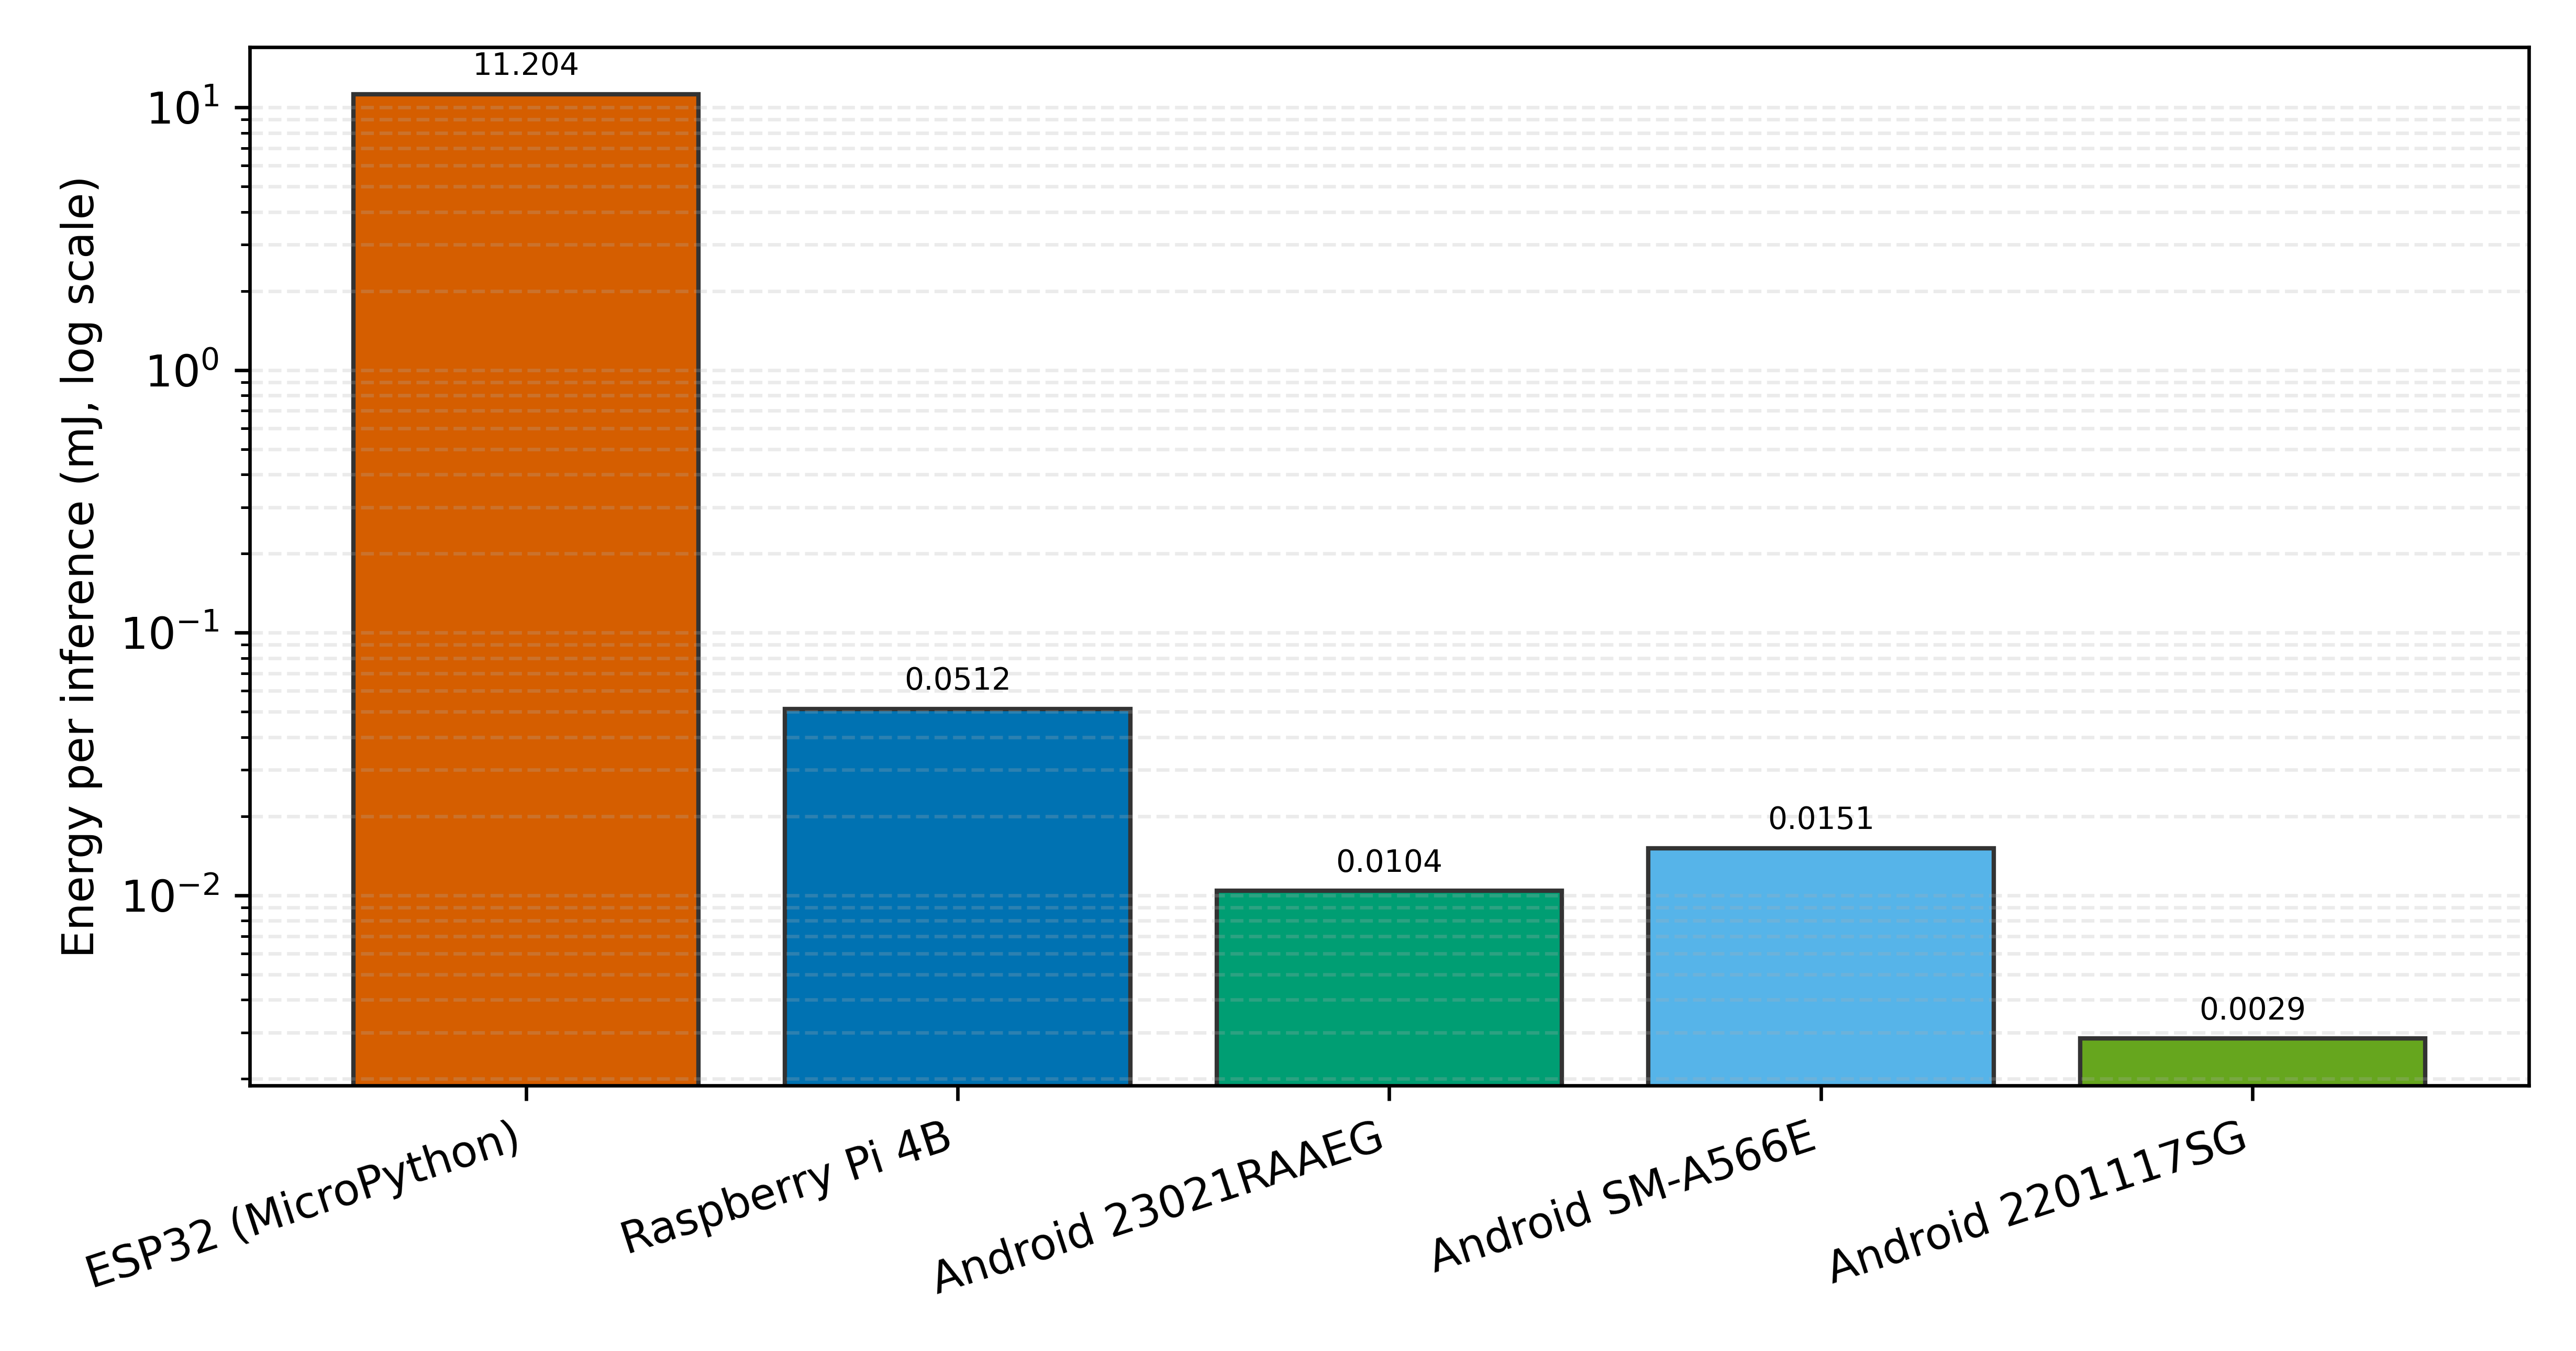
\includegraphics[width=0.98\linewidth]{energy_platforms_bar.png}
\caption{Comparative energy per inference (log scale).}
\label{fig:energy_bar_lnncs}
\end{figure}

Figure~\ref{fig:energy_bar_lnncs} complements Table~\ref{tab:energy_latency} by making the large energy gap between ESP32 and higher-throughput platforms visually explicit on a logarithmic axis. Without log scaling, low-mJ/inf differences among Raspberry Pi and Android devices would be visually compressed; with this scale, relative efficiency differences remain readable and directly comparable.

Figure~\ref{fig:snn_platform_radar_sba} summarizes the multi-criteria deployment envelope and reinforces that there is no single platform dominating all objectives simultaneously. This is important because deployment choice in edge monitoring cannot be reduced to only one number such as throughput or energy per inference. A platform can be very fast and still lose part of its advantage when incremental energy is considered, while a slower platform may remain attractive when hardware simplicity, full offline execution, or lower integration overhead are operational priorities.

The radar view makes this balance easier to interpret by placing throughput, inverse latency, inverse energy, and predictive reference in the same frame. In this representation, Android devices and the Raspberry Pi occupy a broader envelope on response-related axes, which favors denser temporal sampling and more interactive field workflows. ESP32, in contrast, contracts on those axes but remains relevant for sparse and autonomous operation, where low-rate local screening is sufficient and the system must avoid dependence on cloud connectivity or heavier computing stacks. Therefore, the figure should be read as a deployment map rather than as a universal ranking.

\begin{figure}[!t]
\centering
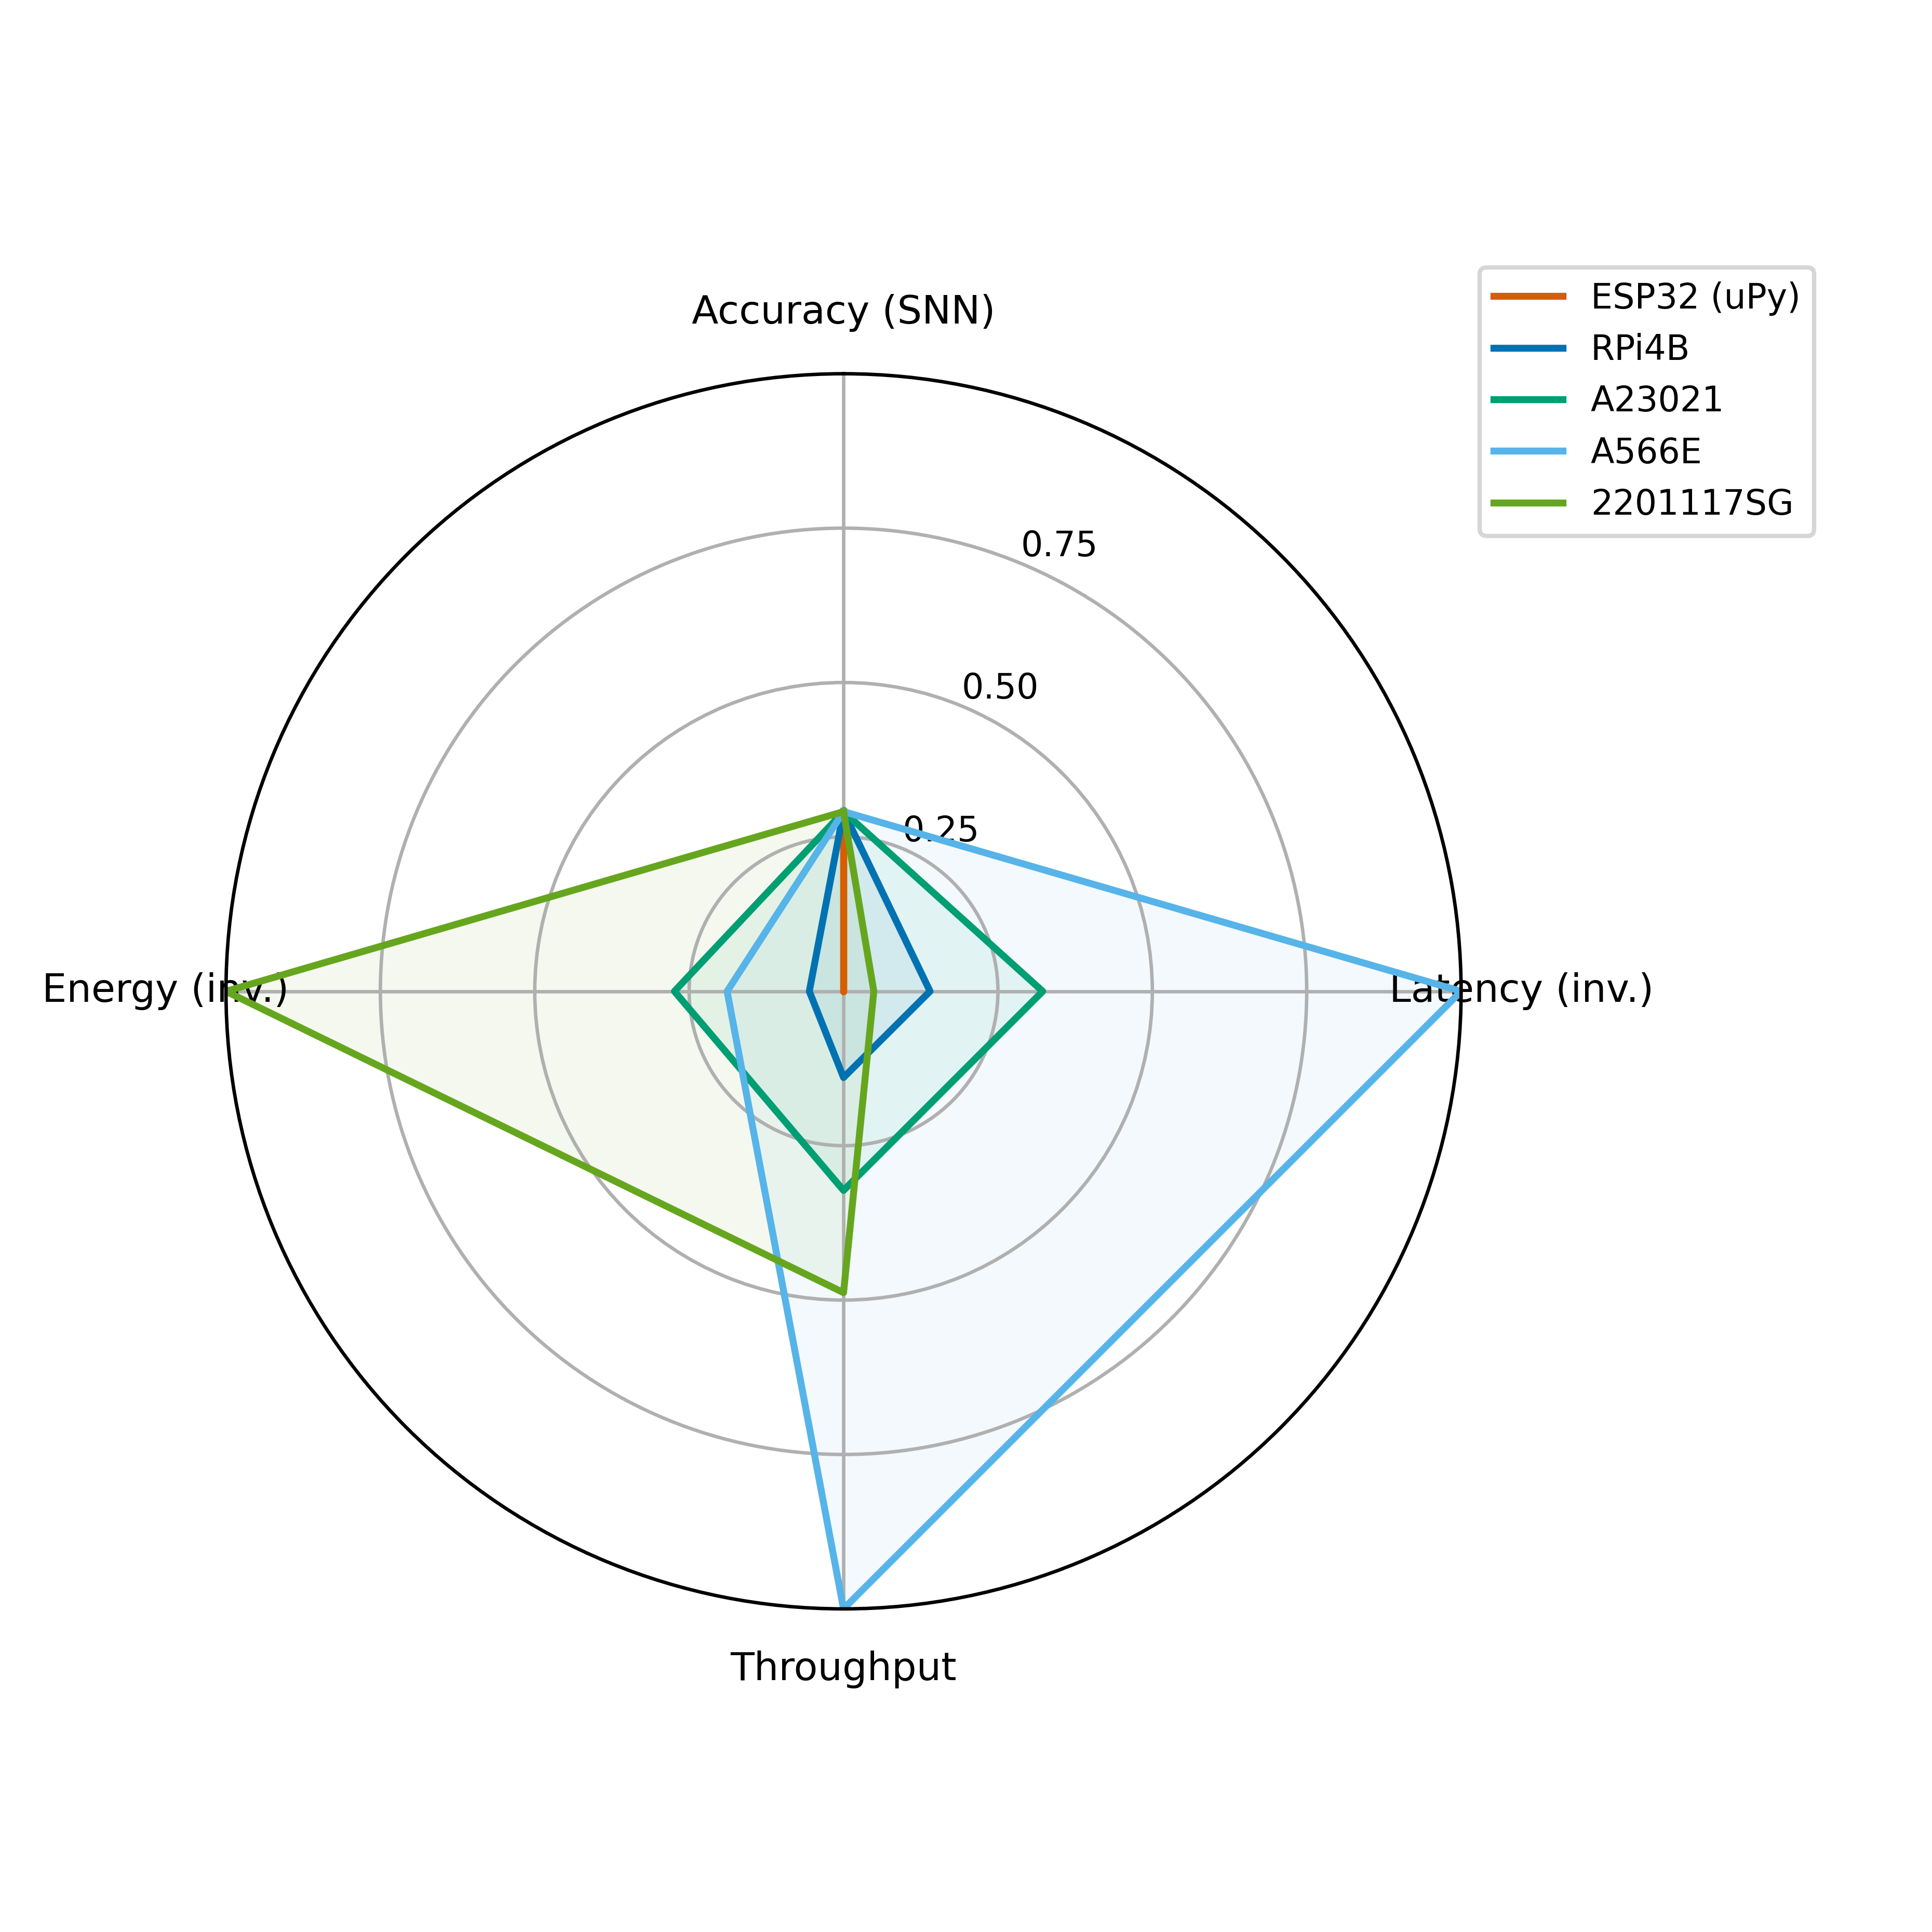
\includegraphics[width=0.90\linewidth]{snn_platform_radar.png}
\caption{SNN deployment comparison across platforms using normalized criteria (throughput, inverse latency, inverse energy, and predictive reference).}
\label{fig:snn_platform_radar_sba}
\end{figure}
